\documentclass{report}
\usepackage[utf8]{inputenc}
\usepackage{mathtools}
\usepackage{amsmath}
\usepackage{amssymb}
\usepackage{enumitem}
\usepackage[export]{adjustbox}
\usepackage{graphicx}
\usepackage{hyperref}
\hypersetup{
    colorlinks=true,
    linkcolor=blue,
    filecolor=magenta,      
    urlcolor=cyan,
    pdftitle={Overleaf Example},
    pdfpagemode=FullScreen,
}
\usepackage{listings}
\usepackage{geometry}
\geometry{
    a4paper,
    total={170mm,257mm},
    left=1in,
    top=1in,
    right=1in,
    bottom=1in,
}
\usepackage[dvipsnames]{xcolor}
\definecolor{codegreen}{rgb}{0,0.6,0}
\definecolor{codegray}{rgb}{0.5,0.5,0.5}
\definecolor{codepurple}{rgb}{0.58,0,0.82}
\definecolor{mygreen}{RGB}{28,172,0} 
\definecolor{mylilas}{RGB}{170,55,241}
\definecolor{backcolour}{rgb}{0.95,0.95,0.92}
\lstdefinestyle{mystyle}{
    backgroundcolor=\color{backcolour},   
    commentstyle=\color{codegreen},
    keywordstyle=\color{blue},
    numberstyle=\tiny\color{codegray},
    stringstyle=\color{codepurple},
    basicstyle=\ttfamily\scriptsize,
    breakatwhitespace=false,         
    breaklines=true,                 
    captionpos=b,                    
    keepspaces=true,                 
    numbers=left,                    
    numbersep=5pt,                  
    showspaces=false,                
    showstringspaces=false,
    showtabs=false,                  
    tabsize=2,
    aboveskip=\medskipamount
}
\lstset{style=mystyle,language=MATLAB, }

\setlength{\parindent}{0pt}

\usepackage{caption}
\usepackage{subcaption}

 \usepackage{array,multirow,graphicx}

\usepackage{tcolorbox}
\tcbuselibrary{skins}

\usepackage{imakeidx}

\usepackage{algorithm}
\usepackage[noend]{algpseudocode}

\usepackage{parskip}
%\setlength{\parskip}{\baselineskip}%
%\setlength{\parindent}{0pt}
\usepackage{booktabs}
\usepackage{amsmath}
\usepackage{amsthm}
\usepackage{bbm}

\makeatletter
\def\thm@space@setup{%
  \thm@preskip=\parskip \thm@postskip=0pt
}

% Math commands
\newenvironment{sysmatrix}[1]
 {\left[\begin{array}{@{}#1@{}}}
 {\end{array}\right]}
\newcommand{\ro}[1]{%
  \xrightarrow{\mathmakebox[\rowidth]{#1}}%
}
\newlength{\rowidth}% row operation width
\newcommand{\vt}[3]{\begin{sysmatrix}{c}#1\\#2\\#3\end{sysmatrix}}
\AtBeginDocument{\setlength{\rowidth}{3em}}
\newcommand\bigzero{\makebox(0,0){\text{\huge0}}}

\newcommand*\Eval[3]{\left.#1\right\rvert_{#2}^{#3}}
\newcommand\norm[1]{\left\lVert#1\right\rVert}

\newcommand{\cov}[1]{\text{Cov}\left(#1\right)}
\newcommand{\ev}[1]{E\left[#1\right]}

\newcommand{\argmin}{\mathop{\mathrm{arg\,min}}\limits}
\newcommand{\argmax}{\mathop{\mathrm{arg\,max}}\limits}


% Theorems + other boxed stuff (adapted from gilles castel)
\makeatother
\usepackage{thmtools}
\usepackage[framemethod=TikZ]{mdframed}
\mdfsetup{skipabove=1em,skipbelow=0em}

\declaretheoremstyle[
    headfont=\bfseries\sffamily\color{ForestGreen!70!black}, 
    notefont=\bfseries\sffamily\color{ForestGreen!70!black}, 
    bodyfont=\normalfont,
    notebraces={( }{ )},
    headpunct={},
    postheadspace=1em,
    mdframed={
        linewidth=2pt,
        rightline=false, topline=false, bottomline=false,
        linecolor=ForestGreen, backgroundcolor=ForestGreen!5,
    }
]{defshaded}

\declaretheoremstyle[
    headfont=\bfseries\sffamily\color{NavyBlue!70!black}, 
    notefont=\bfseries\sffamily\color{NavyBlue!70!black}, 
    bodyfont=\normalfont,
    notebraces={( }{ )},
    headpunct={},
    postheadspace=1em,
    mdframed={
        linewidth=2pt,
        linecolor=NavyBlue
    }
]{egbox}

\declaretheoremstyle[
    headfont=\bfseries\color{RawSienna!70!black}, 
    notefont=\bfseries\color{RawSienna!70!black}, 
    bodyfont=\normalfont,
    notebraces={( }{ )},
    headpunct={},
    postheadspace=1em,
    mdframed={
        linewidth=2pt,
        rightline=false, topline=false, bottomline=false,
        linecolor=RawSienna, backgroundcolor=RawSienna!5,
    }
]{thmshaded}

\declaretheoremstyle[
    headfont=\bfseries\sffamily\color{RawSienna!70!black}, 
    notefont=\bfseries\sffamily\color{RawSienna!70!black}, 
    bodyfont=\normalfont,
    notebraces={( }{ )},
    headpunct={},
    postheadspace=1em,
    mdframed={
        linewidth=2pt,
        rightline=false, topline=false, bottomline=false,
        linecolor=RawSienna
    }
]{thmline}

\declaretheoremstyle[
    headfont=\bfseries\sffamily\color{RawSienna!70!black}, 
    notefont=\bfseries\sffamily\color{RawSienna!70!black}, 
    bodyfont=\normalfont,
    notebraces={( }{ )},
    headpunct={},
    postheadspace=1em,
    mdframed={
        linewidth=2pt,
        rightline=false, topline=false, bottomline=false,
        linecolor=RawSienna, backgroundcolor=RawSienna!1,
    },
    qed=\qedsymbol
]{thmproof}

\theoremstyle{definition}

\declaretheorem[style=defshaded, numbered=no, name=Definition]{definition}
\declaretheorem[style=egbox, numberwithin=chapter, name=Example]{example}
\declaretheorem[style=thmshaded, numberwithin=chapter, name=Theorem]{theorem}
\declaretheorem[style=thmshaded, numberwithin=chapter, sibling=theorem, name=Proposition]{proposition}
\declaretheorem[style=thmshaded, numberwithin=chapter, sibling=theorem, name=Lemma]{lemma}
\declaretheorem[style=thmshaded, numberwithin=chapter, sibling=theorem, name=Corollary]{corollary}
\declaretheorem[style=thmline, numbered=no, name=Remark]{remark}
\declaretheorem[style=thmline, numbered=no, name=Note]{note}

\declaretheorem[style=thmproof, numbered=no, name=Proof]{replacementproof}
\renewenvironment{proof}[1][\proofname]{\vspace{-1.1em}\begin{replacementproof}}{\end{replacementproof}}
\AtBeginEnvironment{proof}{\renewcommand{\qedsymbol}{}}{}{}

\newcommand{\eg}[2]{
    \begin{example}[#1]\phantom{.}\newline#2\end{example}
}
\newcommand{\thm}[2]{
    \begin{theorem}[#1]\phantom{.}\newline#2\end{theorem}
}
\newcommand{\cor}[2]{
    \begin{corollary}[#1]\phantom{.}\newline#2\end{corollary}
}
\newcommand{\lem}[2]{
    \begin{lemma}[#1]\phantom{.}\newline#2\end{lemma}
}
\newcommand{\defn}[2]{
    \begin{definition}[#1]\phantom{.}\newline#2\end{definition}
}


% misc
\newcommand{\shrug}[1][]{%
\begin{tikzpicture}[baseline,x=0.8\ht\strutbox,y=0.8\ht\strutbox,line width=0.125ex,#1]
\def\arm{(-2.5,0.95) to (-2,0.95) (-1.9,1) to (-1.5,0) (-1.35,0) to (-0.8,0)};
\draw \arm;
\draw[xscale=-1] \arm;
\def\headpart{(0.6,0) arc[start angle=-40, end angle=40,x radius=0.6,y radius=0.8]};
\draw \headpart;
\draw[xscale=-1] \headpart;
\def\eye{(-0.075,0.15) .. controls (0.02,0) .. (0.075,-0.15)};
\draw[shift={(-0.3,0.8)}] \eye;
\draw[shift={(0,0.85)}] \eye;
\draw (-0.1,0.2) to [out=15,in=-100] (0.4,0.95); 
\end{tikzpicture}}
\usepackage{xcolor,colortbl}
\usepackage{tikz}
\usetikzlibrary{matrix}
\definecolor{color1}{RGB}{56,108,241}
\definecolor{color2}{RGB}{38,164,66}
\definecolor{color3}{RGB}{216,56,56}
\definecolor{color4}{RGB}{149,52,200}
\definecolor{color5}{RGB}{122,43,26}
\definecolor{color6}{RGB}{42,194,189}
\definecolor{color7}{RGB}{126,126,126}
\definecolor{color8}{RGB}{35,35,35}
\definecolor{unknown}{RGB}{255,255,255}
\definecolor{uncovered}{RGB}{198,198,198}
\definecolor{possible1}{RGB}{218,218,188}
\definecolor{possible2}{RGB}{218,188,218}
\definecolor{possible3}{RGB}{188,218,218}

\newcommand{\cellflex}[2]{\node[fill=#2,minimum width=1cm,minimum height=1cm,text centered] {#1};}
\newcommand{\cellflag}{
\node[fill=unknown,minimum width=1cm,minimum height=1cm] {};
            \draw[fill=red] (-0.15,0.5)--(0.2,0.35)--(-0.15,0.2)--cycle;
            \draw[thick] (-0.15,-0.1)--(-0.15,0.5);
}
\newcommand{\cellzero}{\node[fill=uncovered,minimum width=1cm,minimum height=1cm,text centered] {};}
\newcommand{\cellzeromarked}{\node[fill=uncovered,minimum width=1cm,minimum height=1cm,text centered] {\LARGE 0};}
\newcommand{\cellone}{\node[fill=uncovered,minimum width=1cm,minimum height=1cm,text centered] {\textcolor{color1}{\LARGE \textbf{1}}};}
\newcommand{\celltwo}{\node[fill=uncovered,minimum width=1cm,minimum height=1cm,text centered] {\textcolor{color2}{\LARGE \textbf{2}}};}
\newcommand{\cellthree}{\node[fill=uncovered,minimum width=1cm,minimum height=1cm,text centered] {\textcolor{color3}{\LARGE \textbf{3}}};}
\newcommand{\cellfour}{\node[fill=uncovered,minimum width=1cm,minimum height=1cm,text centered] {\textcolor{color4}{\LARGE \textbf{4}}};}
\newcommand{\cellfive}{\node[fill=uncovered,minimum width=1cm,minimum height=1cm,text centered] {\textcolor{color5}{\LARGE \textbf{5}}};}
\newcommand{\cellsix}{\node[fill=uncovered,minimum width=1cm,minimum height=1cm,text centered] {\textcolor{color6}{\LARGE \textbf{6}}};}
\newcommand{\cellseven}{\node[fill=uncovered,minimum width=1cm,minimum height=1cm,text centered] {\textcolor{color7}{\LARGE \textbf{7}}};}
\newcommand{\celleight}{\node[fill=uncovered,minimum width=1cm,minimum height=1cm,text centered] {\textcolor{color8}{\LARGE \textbf{8}}};}
\newcommand{\cellunk}{\node[fill=unknown,minimum width=1cm,minimum height=1cm,text centered] {};}
\newcommand{\celldc}{\node[fill=uncovered,minimum width=1cm,minimum height=1cm,text centered] {\LARGE$\ast$};}
\newcommand{\celludc}{\node[fill=unknown,minimum width=1cm,minimum height=1cm,text centered] {\LARGE$\ast$};}
\newcommand{\cellsafe}{\node[fill=color2,minimum width=1cm,minimum height=1cm,text centered] {};}
\newcommand{\cellmine}{\node[fill=color3,minimum width=1cm,minimum height=1cm,text centered] {};}
\newcommand{\cellmsm}[2]{\node[fill=#2,minimum width=1cm,minimum height=1cm,text centered] {\LARGE \textbf{#1}};}
\newcommand{\cellvar}[1]{\node[fill=uncovered,minimum width=1cm,minimum height=1cm,text centered] {\LARGE \textbf{#1}};}
\newcommand{\celllabel}[1]{\node[fill=unknown,minimum width=1cm,minimum height=1cm,text centered] {\LARGE $#1$};}

\NewDocumentEnvironment{minesweeperboard}{b}{%
    \begin{tikzpicture}%
    \matrix [matrix of nodes,anchor=base,text depth=0.3cm,text height=0.7cm,text width=1cm,every node/.style={draw},ampersand replacement=\&]{#1};
    \end{tikzpicture}%
}{}
%\usepackage{tikz-minesweeper}
\makeindex[columns=3, title=Index]

\title{A Human's Guide to Minesweeper}
\author{}
\date{April 2023}

\begin{document}

\maketitle
\newpage

\section*{TL;DR if you're new}

This is minesweeper\\
\begin{figure}[h]
    \centering
    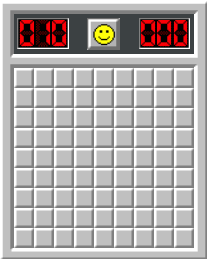
\includegraphics{figures/1/empty_board.PNG}
\end{figure}

This is a mine. They occupy some spaces of the board.\\
\begin{figure}[h]
    \centering
    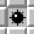
\includegraphics{figures/1/mine.PNG}
\end{figure}

Play by clicking squares. Numbers say how many of the neighboring squares (including diagonals) have mines.\\
\begin{figure}[h]
    \centering
    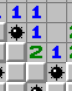
\includegraphics{figures/1/example.PNG}
\end{figure}

Win by uncovering all squares without mines.\\


\vspace{10em}
{\huge DO NOT READ ANY FURTHER}\\

I strongly encourage you to play and learn the game yourself. IMO this is the best way to have fun playing minesweeper.


\newpage

\tableofcontents
\newpage

\chapter{Introduction}

\subsubsection*{Who am I?}

I am not among the elites of minesweeper. As of writing, my best time on expert difficulty is 80 seconds\footnote{My minesweeper.online profile: \url{https://minesweeper.online/player/1896875}}, leaving me much room to improve. I do, however, love playing this game.\\

I discovered minesweeper in 3rd grade. My parents got me an old IBM ThinkPad 20M to do essays and nothing else. For gaming, I was restricted to the 4 games that came with Windows 98: Solitaire, Freecell, Hearts, and Minesweeper. At the time, I barely understood the rules or strategy, and I was not allowed free time on the internet to learn either. I got more into minesweeper towards the end of high school, when I inherited the family laptop nobody bothered to use because the case was so broken beyond repair. Unable to effectively play any other games on it, I turned to playing the built in Windows 7 minesweeper to pass time. Being more mature, I actually sat down and learned the game. Using the laptop trackpad, I was able to clear the expert difficulty on a regular basis. During college, I discovered minesweeper.online, and started to actually try to get better at the game. Even as I got to build my own PC capable of playing higher fidelity games, minesweeper was a game I'd always play during the frequent gaps I procrastinated on assignments.\\

Requiring fast-paced logic balanced with quick risk assessment, playing minesweeper has become one of my favorite past-times to put me into a pleasant state of flow. It is my hope that more people will be able to enjoy this game as much as I do.\\

\subsubsection*{What is this?}

This document is an unnecessarily long guide on minesweeper. As a graduate student in engineering, I find myself typesetting a lot of homework and papers in LaTeX, so I thought it'd be fun to put my thoughts on minesweeper in a similar format. There are already a fair number of papers exploring the math of minesweeper\footnote{Collection of math papers on minesweeper \url{https://minesweepergame.com/math-papers.php}}, however the math I present in this document in completely in the service of the player, aiming to root the decisions that can be made in minesweeper within a mathematical framework. My goal is to assemble and formalize everything I've learned about minesweeper, from the patterns beginners learn to the guessing strategies I've developed based on computer simulations, into a single document in the most comprehensive way possible. To reiterate, this document is just for fun.\\

\subsubsection*{What is this not?}

While this is a strategy guide, this is not a guide by example. While there are examples in this document (when I remember to add them in), the goal is to develop a framework for analysis that works in arbitrary positions. There are plenty of great guides that are more visual\footnote{Lowenthal made a 117 page guide (I hope to do longer eventually) \\ \url{https://minesweepergame.com/file/Minesweeper-JohnLowenthal-1992.pdf}}\footnote{minesweeper.com also has a lot of guides\url{https://minesweeper.online/help/guides}}, but I hope to insert some mathematical rigor into the analysis of minesweeper that seems to be missing from other guides.\\

\subsubsection*{Who is this for?}

Mostly myself. However, I'd be overjoyed if anyone else read over this document and either learned something or otherwise found it enjoyable. I aim to break down the game to the most basic level, so players of any skill level will be able to take away something from this document.\\

\subsubsection*{Why is this document so confusing?}

I found the motivation to write this document an interesting contradiction. I want the ideas in this document to ultimately serve as tips to improve human play for minesweeper. However, after skimming this document a person will quickly realize that this document is not very human readable.\\

My intention is not to gatekeep the ideas I lay out. Quite the contrary. However, one concept ends up building up on another, and it is very difficult to print short explanations without setting up notation and frameworks to abbreviate thought. I'm well aware of the pedagogical challenges math faces, and I try my best to take things really slow, step by step. Section 2 was an attempt to alleviate these notational problems, by hiding away much of the math and summarize tips derived from the rest of the document, that can be immediately useful to novice to intermediate players.\\

\subsubsection*{I found something that should be changed/added in this document.}

Unfortunately I'm only human, so I'm very prone to errors. If any are found, feel free to DM me on minesweeper online\footnote{My minesweeper.online profile again: \url{https://minesweeper.online/player/1896875}}. Also, my knowledge of the existing works on the math behind minesweeper remains limited. If there are any works that expands on an idea in a more thorough way than I do, I would like to know so I can read it, redirect whoever is reading this to them, and maybe reference their ideas in future edits.\\

\subsubsection*{How is this document structured?}

Section 2 starts out with the very basics that are typically picked up within the first few days of playing. For players already familiar with the game, no new information will likely be learned here. Section 3 dives deeper into the clicks that you can through pure logic. In this section, the mathematical framework I use to describe minesweeper is also introduced. Section 4 looks at the problem of optimal guessing in the framework of probability. Section 5 takes a side step to look at efficiency, which is given by solving a board in the least amount of click possible. Section 6 steps away from meat space entirely to see how a computer can approach minesweeper, and to see what insights computer play can give regarding human play. Finally, section 7 looks at various goals of playing minesweeper and how strategies may differ between each goal.\\

\subsubsection*{Acknowledgements}

Shout out to the kind people at minesweeper online and their great collection of guides\footnote{\url{https://minesweeper.online/help/guides}}. Shoutout to MSCoach for answering some of my questions regarding his solver algorithm. Also shoutout to my brother who I inundated with snippets of this document although he understood absolutely none of it.\\
\newpage

\chapter{Basics}
Minesweeper may seem intimidating for a beginner. This section is a gentle introduction to the mechanics of the game, followed by a simple set of tools to allow beginners to get their first wins. To remain beginner friendly, math will be kept at a minimum in this section. By the end of this section readers should be able to clear intermediate level boards with confidence in their decisions, and be able to tackle expert boards with some success.\\

\section{How to Play}

\subsubsection*{Controls}
Controls are largely dependent on the platform you decide to play minesweeper on. The following are universal actions and the keybinds I tend to find associated with them when playing with mouse and keyboard.
\begin{itemize}
    \item \textbf{Start a new game}: Click the smiley face, F2 (also Spacebar for minesweeper.online)
    \item \textbf{Clear}: Left-Click
    \item \textbf{Flag/Unflag}: Right-Click
    \item \textbf{Chording}: Left+Right-Click, Middle-Click (also Left-Click for minesweeper.online)
\end{itemize}
Note: For some versions, right clicking will cycle through a flag, a ? question mark, and an unmarked square. If able, I recommend turning off ``Marks (?)" in the settings, as question marks don't serve too much utility while playing.\\


\subsubsection*{Clearing Squares}
Left-clicking on a square is a commitment. You are declaring, ``I swear on my life that there is no mine on this square." Should you left-click on a square containing a mine.\\

\textbf{Clearing}\index{Clear} an unknown square checks the value of the square. Four things can happen when you clear a square:
\begin{enumerate}
    \item There is no mine in the square, and a number appears. This number indicates the number of mines in the eight neighboring squares (or less if the square is on an edge).
    \item There is no mine in the square, and many numbers appear. This is called an \textbf{opening}\index{Opening}. An opening occurs when there are no mines in the square you click, as well as the squares neighboring the square you click. This is an effective ``0" number, but games typically leave the square blank, and automatically clears all the squares around the zeros recursively until no more squares can be cleared.
    \item You click a mine. You are dead.
    \item You've cleared the last square that's not a mine. You've won the game
\end{enumerate}
\begin{figure}[h]
    \centering
    \begin{subfigure}[t]{0.2\textwidth}
        \centering
        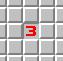
\includegraphics[width=0.8\linewidth]{figures/2.1/single}
        \caption{Single number}
    \end{subfigure}
    \begin{subfigure}[t]{0.2\textwidth}
        \centering
        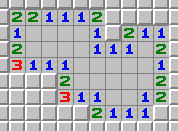
\includegraphics[width=0.8\linewidth]{figures/2.1/opening}
        \caption{Opening}
    \end{subfigure}
    \begin{subfigure}[t]{0.2\textwidth}
        \centering
        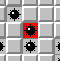
\includegraphics[width=0.8\linewidth]{figures/2.1/mine}
        \caption{Mine}
    \end{subfigure}
    \begin{subfigure}[t]{0.2\textwidth}
        \centering
        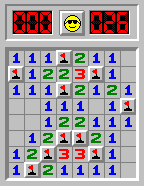
\includegraphics[width=0.8\linewidth]{figures/2.1/win}
        \caption{Win (Note the sunglasses on the smiley face}
    \end{subfigure}
    \caption{The four possible scenarios when clearing a square}
\end{figure}


\subsubsection*{The First Click}
The game starts when you clear the first square. The first left-click you make is guaranteed to never be a mine. Leaving the details for future sections (Section \ref{sec:simple_guessing}), basic rule of thumb is to \textbf{choose a corner for your first click}. The idea is to hope for an opening on your first click that will minimize the amount of needed guessing. Hand waving a lot, corners are a good choice because it only has 3 neighbors, giving it the high odd of having no neighboring mines, leading to an opening. If the first corner does not lead to a sufficient opening, clicking on other corners is also an okay idea (more on this later).\\


\subsubsection*{Use Flags to Mark Where You Think Mines Are}
\textbf{Flags}\index{Flag} can be placed on the grid by right-clicking a square. This will decrement the mine counter. Flags can still be placed on squares without a mine, and this will still decrease the mine counter. Flags do NOT verify that a mine is at a given square. They are simply a useful tool the player can use to mark possible mine locations.\\

Flagging is more than just a visual aid. They can be used for chording (discussed below), minecounting (Section 3.4), and for preventing possible misclicks onto the mine. For beginners and anyone not playing for speed, I highly recommend to \textbf{place a flag at every location you know there is a mine}.\\

Do note that there exists a ``No Flag" playstyle where players intentionally play without flags. This can improve speed in some cases since you are not using extraneous clicks to flag obvious mines. In section 5, we'll find that a hybrid approach where only some mines are flagged may actually be the fastest strategy. In my opinion, for higher difficulties expert and above, not flagging at all is psychotic, but if this is you, you do you.\\


\subsubsection*{Chording}
\textbf{Chording}\index{Chording} is a technique where you click a number with the number's number of flags adjacent to it (we'll call this a \textbf{chordable} number). This clears all the squares around the number you click (and if a surrounding square is an opening, a recursive clearing is performed).\\

Chording can be normally be performed with either a middle-click, or by pressing left and right-click at the same time. As chording typically follows placing a flag, you can keep holding the right-click from placing the flag, and left-click the fulfilled number next to the flag to chord. However, when the platform allows, sometimes just left-clicking the fulfilled number will also chord.\\

If used correctly, chording can greatly reduce the number of clicks you use. Like flagging, chording all the time is usually not optimal for speed. However, advanced players can use chording to speed up clears. For beginners, chording is hardly necessary to know, but I personally used chording a lot when learning. Chording reduces the number of raw left-clicks you perform on the unknown squares, reducing possible misclick encouters.\\

\section{Basic Patterns}\label{sec:basic-patterns}

\begin{table}[h]
    \centering
    \begin{tabular}{|c|p{0.7\linewidth}|}\hline
         \begin{minipage}{1cm}\begin{minesweeperboard}\cellunk\\\end{minesweeperboard}\end{minipage}& Unknown square: May or may not contain a mine \\\hline
         \begin{minipage}{1cm}\begin{minesweeperboard}\cellflag\\\end{minesweeperboard}\end{minipage}& Known mine\\\hline
         \begin{minipage}{1cm}\begin{minesweeperboard}\cellzero\\\end{minesweeperboard}\end{minipage}& Zero square (opening): Does not contain a mine and adjacent squares do not contain a mine\\\hline
         \begin{minipage}{1.45cm}\begin{minesweeperboard}\cellone\\\end{minesweeperboard}\end{minipage}...\begin{minipage}{1.5cm}\begin{minesweeperboard}\celleight\\\end{minesweeperboard}\end{minipage}& Numbered square: Does not contain a mine and \# adjacent squares contain a mine \\\hline
         \begin{minipage}{1cm}\begin{minesweeperboard}\celludc\\\end{minesweeperboard}\end{minipage}& Unknown Don't Care (UDC) square: May contain a mine, but we don't care if it contains a mine, or what numerical value it has if it doesn't contain a mine\\\hline
         \begin{minipage}{1cm}\begin{minesweeperboard}\celldc\\\end{minesweeperboard}\end{minipage}& Don't Care (DC) square: Does not contain a mine, but we don't care about its numerical value\\\hline
         \begin{minipage}{1cm}\begin{minesweeperboard}\cellsafe\\\end{minesweeperboard}\end{minipage}& Safe square: It can be inferred that there are no mines here; should be cleared\\\hline
         \begin{minipage}{1cm}\begin{minesweeperboard}\cellmine\\\end{minesweeperboard}\end{minipage}& Unsafe square: It can be inferred that there is a mine here; can be flagged\\\hline
         \begin{minipage}{1cm}\begin{minesweeperboard}\cellmsm{$A_x$}{possible1}\\\end{minesweeperboard}\end{minipage}& Mutually Shared Mine (MSM) squares: All squares containing the same letter share a possibility of having $x$ number of mines. The existence of $x$ mines within these squares excludes the possibility of the others containing a mine\\\hline
         \begin{minipage}{1cm}\begin{minesweeperboard}\celllabel{a}\\\end{minesweeperboard}\end{minipage}& Labeled square: An unknown square with a name for ease of reference in explanations\\\hline
    \end{tabular}
    \caption{Diagram Key}
    \label{tab:diagram_key}
\end{table}

So how do you know which squares to clear and which squares to flag? While I encourage beginners to exercise basic logic to figure out which squares deserve which click, this section will provide a quick cheat-sheet of common simple patterns that occur in play. These patterns are ordered from most simple/common, to the slightly more obscure. This section will not contain all commonly known patterns, but these are the patterns I personally think warrant memorization for a beginner.\\

Section 3 will go over these patterns (and more) in more detail. For now, these patterns can be taken for granted, and will typically be enough to solve nearly all intermediate boards and some expert boards.\\

Before discussing these patterns, a key for the figures used will have to be introduced. A key for the diagrams used in this document is shown in Table \ref{tab:diagram_key} Most of these will be identical the the notation used in game. The first six rows in the table will depict the state of the board. Green cells and red cells indicate areas where conclusions can be drawn hence can be either cleared (green) or flagged (red). The last row describes cells where it is unknown if a mine exists in any individual square, but it is known that mines exists among the squares marked by the same letter.\\

Board diagrams show only a subset of a board, and are assumed to extend infinitely in all directions unless otherwise stated. Squares beyond the edges of the board can be imagined as unknown don't care (UDC) squares.\\


\subsection{Local Counting Patterns}
\subsubsection*{All Mines}
When the number of unknown spaces surround a number equals that number, one can infer that all those spaces must be mines.

\eg{1-Corner}{
\begin{center}
    \begin{minipage}{0.2\linewidth}\centering\resizebox{1\linewidth}{!}{\begin{minesweeperboard}
        \cellzero \& \celldc \& \cellunk\\
        \cellzero \& \cellone \& \celldc\\
        \cellzero \& \cellzero \& \cellzero\\
    \end{minesweeperboard}}\end{minipage}{\huge$\Rightarrow$}
    \begin{minipage}{0.2\linewidth}\centering\resizebox{1\linewidth}{!}{\begin{minesweeperboard}
        \cellzero \& \celldc \& \cellmine\\
        \cellzero \& \cellone \& \celldc\\
        \cellzero \& \cellzero \& \cellzero\\
    \end{minesweeperboard}}\end{minipage}{\huge$\sim$}
    \begin{minipage}{0.2\linewidth}\centering\resizebox{1\linewidth}{!}{\begin{minesweeperboard}
        \cellzero \& \celldc \& \cellflag\\
        \cellzero \& \cellone \& \celldc\\
        \cellzero \& \cellzero \& \cellzero\\
    \end{minesweeperboard}}\end{minipage}
\end{center}

This is a classical situation where the location of a mine can easily be determined.
}

\eg{Common ``All Mines" Patterns}{
\begin{center}
    \begin{tabular}{cc}
        \begin{minipage}{0.2\linewidth}\centering\resizebox{1\linewidth}{!}{\begin{minesweeperboard}
            \cellzero \& \celldc \& \celldc\\
            \cellzero \& \celltwo \& \cellunk\\
            \cellzero \& \celldc \& \cellunk\\
        \end{minesweeperboard}}\end{minipage}{\huge$\Rightarrow$}
        \begin{minipage}{0.2\linewidth}\centering\resizebox{1\linewidth}{!}{\begin{minesweeperboard}
            \cellzero \& \celldc \& \celldc\\
            \cellzero \& \celltwo \& \cellmine\\
            \cellzero \& \celldc \& \cellmine\\
        \end{minesweeperboard}}\end{minipage} & 
        
        \begin{minipage}{0.2\linewidth}\centering\resizebox{1\linewidth}{!}{\begin{minesweeperboard}
            \cellzero \& \celldc \& \cellunk\\
            \cellzero \& \cellthree \& \cellunk\\
            \cellzero \& \celldc \& \cellunk\\
        \end{minesweeperboard}}\end{minipage}{\huge$\Rightarrow$}
        \begin{minipage}{0.2\linewidth}\centering\resizebox{1\linewidth}{!}{\begin{minesweeperboard}
            \cellzero \& \celldc \& \cellmine\\
            \cellzero \& \cellthree \& \cellmine\\
            \cellzero \& \celldc \& \cellmine\\
        \end{minesweeperboard}}\end{minipage}\\
        
        \begin{minipage}{0.2\linewidth}\centering\resizebox{1\linewidth}{!}{\begin{minesweeperboard}
            \celldc \& \cellunk \& \cellunk\\
            \celldc \& \cellfour \& \cellunk\\
            \cellzero \& \celldc \& \cellunk\\
        \end{minesweeperboard}}\end{minipage}{\huge$\Rightarrow$}
        \begin{minipage}{0.2\linewidth}\centering\resizebox{1\linewidth}{!}{\begin{minesweeperboard}
            \celldc \& \cellmine \& \cellmine\\
            \celldc \& \cellfour \& \cellmine\\
            \cellzero \& \celldc \& \cellmine\\
        \end{minesweeperboard}}\end{minipage} & 
        
        \begin{minipage}{0.2\linewidth}\centering\resizebox{1\linewidth}{!}{\begin{minesweeperboard}
            \cellunk \& \cellunk \& \cellunk\\
            \celldc \& \cellfive \& \cellunk\\
            \cellzero \& \celldc \& \cellunk\\
        \end{minesweeperboard}}\end{minipage}{\huge$\Rightarrow$}
        \begin{minipage}{0.2\linewidth}\centering\resizebox{1\linewidth}{!}{\begin{minesweeperboard}
            \cellmine \& \cellmine \& \cellmine\\
            \celldc \& \cellfive \& \cellmine\\
            \cellzero \& \celldc \& \cellmine\\
        \end{minesweeperboard}}\end{minipage}
    \end{tabular}

    These are some more common situations where the location of mines can easily be deduced. 
\end{center}
}

As the only action that can be performed with this pattern is flagging, no new information is actually obtained from this pattern, but placing flags following this pattern greatly helps with the visualization of the known information regarding the board.\\

\newpage
\subsubsection*{Mine Reduction (Chordables)}
When a numbered cell is adjacent to a number of known mines (flags or a complete set of MSM squares), the number of mines can be subtracted from the known number and logic can be applied as normal, treating the known mines as don't care (DC) squares.\\

If a mine reduction reduces a number to 0 (i.e. the number of mines around a numbered square equals the number in the square), all neighboring cells to the number can be cleared. If the known mines are explicitly marked with flags, the numbered square can be clicked to perform a chord.

\eg{Mine Reduction}{
\begin{center}
    \begin{minipage}{0.2\linewidth}\centering\resizebox{1\linewidth}{!}{\begin{minesweeperboard}
        \cellunk \& \cellunk \& \cellunk\\
        \celldc \& \celltwo \& \celldc\\
        \celldc \& \cellflag \& \celldc\\
    \end{minesweeperboard}}\end{minipage}{\huge$\sim$}
    \begin{minipage}{0.2\linewidth}\centering\resizebox{1\linewidth}{!}{\begin{minesweeperboard}
        \cellunk \& \cellunk \& \cellunk\\
        \celldc \& \cellone \& \celldc\\
        \celldc \& \celldc \& \celldc\\
    \end{minesweeperboard}}\end{minipage}{\huge$\sim$}
    \begin{minipage}{0.2\linewidth}\centering\resizebox{1\linewidth}{!}{\begin{minesweeperboard}
        \cellmsm{$A_1$}{possible1} \& \cellmsm{$A_1$}{possible1} \& \cellmsm{$A_1$}{possible1}\\
        \celldc \& \cellone \& \celldc\\
        \celldc \& \celldc \& \celldc\\
    \end{minesweeperboard}}\end{minipage}
\end{center}
Since there is one known mine adjacent to the 2, the 2 can be thought of as a 1. From there, no more action can be taken, but it can be concluded that the remaining three unknown squares mutually contain one mine.
}

\eg{Mine Reduction into Chordable}{
\begin{center}
    \begin{minipage}{0.2\linewidth}\centering\resizebox{1\linewidth}{!}{\begin{minesweeperboard}
        \cellunk \& \cellflag \& \cellunk\\
        \celldc \& \celltwo \& \cellunk\\
        \cellzero \& \celldc \& \cellflag\\
    \end{minesweeperboard}}\end{minipage}{\huge$\sim$}
    \begin{minipage}{0.2\linewidth}\centering\resizebox{1\linewidth}{!}{\begin{minesweeperboard}
        \cellunk \& \celldc \& \cellunk\\
        \celldc \& \cellzeromarked \& \cellunk\\
        \cellzero \& \celldc \& \celldc\\
    \end{minesweeperboard}}\end{minipage}{\huge$\Rightarrow$}
    \begin{minipage}{0.2\linewidth}\centering\resizebox{1\linewidth}{!}{\begin{minesweeperboard}
        \cellsafe \& \celldc \& \cellsafe\\
        \celldc \& \cellzeromarked \& \cellsafe\\
        \cellzero \& \celldc \& \celldc\\
    \end{minesweeperboard}}\end{minipage}{\huge$\sim$}
    \begin{minipage}{0.2\linewidth}\centering\resizebox{1\linewidth}{!}{\begin{minesweeperboard}
        \cellsafe \& \cellflag \& \cellsafe\\
        \celldc \& \celltwo \& \cellsafe\\
        \cellzero \& \celldc \& \cellflag\\
    \end{minesweeperboard}}\end{minipage}
\end{center}
An example of a case where mine reduction reduces the number to zero. In this case, all neighbors of the reduced number can safely be cleared or chorded. More often than not, the middle two steps are not actually visualized since it's not difficult to count the number of mines around a square.
}

\eg{Mine Reduction with Mutually Shared Mine Squares}{
\begin{center}
    \begin{minipage}{0.2\linewidth}\centering\resizebox{1\linewidth}{!}{\begin{minesweeperboard}
        \cellunk \& \cellunk \& \cellunk\\
        \cellunk \& \cellthree \& \cellunk\\
        \celldc \& \cellthree \& \cellunk\\
        \cellzero \& \celldc \& \cellflag\\
    \end{minesweeperboard}}\end{minipage}{\huge$\sim$}
    \begin{minipage}{0.2\linewidth}\centering\resizebox{1\linewidth}{!}{\begin{minesweeperboard}
        \cellunk \& \cellunk \& \cellunk\\
        \cellmsm{$A_2$}{possible1} \& \cellthree \& \cellmsm{$A_2$}{possible1}\\
        \celldc \& \celltwo \& \cellmsm{$A_2$}{possible1}\\
        \cellzero \& \celldc \& \celldc\\
    \end{minesweeperboard}}\end{minipage}{\huge$\sim$}
    \begin{minipage}{0.2\linewidth}\centering\resizebox{1\linewidth}{!}{\begin{minesweeperboard}
        \cellmsm{$B_1$}{possible2} \& \cellmsm{$B_1$}{possible2} \& \cellmsm{$B_1$}{possible2}\\
        \celldc \& \cellone \& \celldc\\
        \celldc \& \celldc \& \celldc\\
        \cellzero \& \celldc \& \celldc\\
    \end{minesweeperboard}}\end{minipage}{\huge$\sim$}
    \begin{minipage}{0.2\linewidth}\centering\resizebox{1\linewidth}{!}{\begin{minesweeperboard}
        \cellmsm{$B_1$}{possible2} \& \cellmsm{$B_1$}{possible2} \& \cellmsm{$B_1$}{possible2}\\
        \cellmsm{$A_2$}{possible1} \& \cellthree \& \cellmsm{$A_2$}{possible1}\\
        \celldc \& \cellthree \& \cellmsm{$A_2$}{possible1}\\
        \cellzero \& \celldc \& \cellflag\\
    \end{minesweeperboard}}\end{minipage}
\end{center}
A more complicated example illustrating how mutually shared mine (MSM) squares can also be used in mine subtraction. Note that all the MSM squares in the same group must be adjacent to the number you want to reduce.  This concept will be key in understanding the next two patterns.
}


\subsection{Core Patterns}
There are two core patterns, the 1-1 pattern and the 1-2 pattern. For someone discovering minesweeper strategy on their own, these will often be among the first patterns they discover. In their simplest form, these patterns are a bit restricting, but the logic used to discover them lead to some nice generalized patterns that can still be recognized at a glance. In a Section 3, it will be discussed how these two patterns are actually the same pattern.
\subsubsection*{1-1 Pattern}
When encountering a horizontally or vertically adjacent numbers with the same value, this is a common tool. The 1-1 pattern traditionally has the following form:

\begin{center}
    \begin{minipage}{0.2\linewidth}\centering\resizebox{1\linewidth}{!}{\begin{minesweeperboard}
        \celldc \& \cellunk \& \cellunk \& \cellsafe\\
        \celldc \& \cellone \& \cellone \& \celldc\\
        \celldc \& \cellzero \& \cellzero \& \cellzero\\
    \end{minesweeperboard}}\end{minipage}
\end{center}

While most commonly occurring on the straight edge of an opening, it can be generalized to the following

\thm{Generalized 1-1 Pattern}{\index{1-1 Pattern!grid}
If two numbered cells with the same number $X$ are adjacent and one side is all clear (left side in depiction), the other side is clear.
\begin{center}
    \begin{minipage}{0.2\linewidth}\centering\resizebox{1\linewidth}{!}{\begin{minesweeperboard}
        \celldc \& \cellunk \& \cellunk \& \cellsafe\\
        \celldc \& \cellvar{$X$} \& \cellvar{$X$} \& \cellsafe\\
        \celldc \& \celludc \& \celludc \& \cellsafe\\
    \end{minesweeperboard}}\end{minipage}
\end{center}
}

where $X$ is any number between 1 and 3. The reasoning behind this pattern can be seen as a sequence of mine reductions as follows:

\begin{center}
    \begin{minipage}{0.2\linewidth}\centering\resizebox{1\linewidth}{!}{\begin{minesweeperboard}
        \celldc \& \cellunk \& \cellunk \& \cellunk\\
        \celldc \& \cellvar{$X$} \& \cellvar{$X$} \& \cellunk\\
        \celldc \& \celludc \& \celludc \& \cellunk\\
    \end{minesweeperboard}}\end{minipage}{\huge$\sim$}
    \begin{minipage}{0.2\linewidth}\centering\resizebox{1\linewidth}{!}{\begin{minesweeperboard}
        \celldc \& \cellmsm{$A_X$}{possible1} \& \cellmsm{$A_X$}{possible1} \& \cellunk\\
        \celldc \& \cellvar{$X$} \& \cellvar{$X$} \& \cellunk\\
        \celldc \& \cellmsm{$A_X$}{possible1} \& \cellmsm{$A_X$}{possible1} \& \cellunk\\
    \end{minesweeperboard}}\end{minipage}{\huge$\Rightarrow$}
    \begin{minipage}{0.2\linewidth}\centering\resizebox{1\linewidth}{!}{\begin{minesweeperboard}
        \celldc \& \celldc \& \celldc \& \cellsafe\\
        \celldc \& \cellvar{0} \& \cellvar{0} \& \cellsafe\\
        \celldc \& \celldc \& \celldc \& \cellsafe\\
    \end{minesweeperboard}}\end{minipage}{\huge$\sim$}
    \begin{minipage}{0.2\linewidth}\centering\resizebox{1\linewidth}{!}{\begin{minesweeperboard}
        \celldc \& \cellunk \& \cellunk \& \cellsafe\\
        \celldc \& \cellvar{$X$} \& \cellvar{$X$} \& \cellsafe\\
        \celldc \& \celludc \& \celludc \& \cellsafe\\
    \end{minesweeperboard}}\end{minipage}
\end{center}

The left $X$ makes all adjacent unknown squares into an MSM group. since the MSM group is also adjacent to the right $X$, the right $X$ can be reduced to a zero, hence all the remaining unknown squares adjacent to the right $X$ can safely be cleared.

\eg{1-1 Pattern in $2\times3$ corner opening}{
\begin{center}
    \begin{tabular}{cc}
        \begin{minipage}{0.25\linewidth}\centering\resizebox{1\linewidth}{!}{\begin{minesweeperboard}
            \celldc \& \celldc \& \celldc \& \celldc \& \celldc\\
            \celldc \& \cellzero \& \cellzero \& \cellone \& \cellunk\\
            \celldc \& \cellone \& \cellone \& \cellone \& \cellunk\\
            \celldc \& \cellunk \& \cellunk \& \cellunk \& \cellunk\\
        \end{minesweeperboard}}\end{minipage}{\huge$\Rightarrow$}
        \begin{minipage}{0.25\linewidth}\centering\resizebox{1\linewidth}{!}{\begin{minesweeperboard}
            \celldc \& \celldc \& \celldc \& \celldc \& \celldc\\
            \celldc \& \cellzero \& \cellzero \& \cellone \& \cellunk\\
            \celldc \& \cellone \& \cellone \& \cellone \& \cellunk\\
            \celldc \& \cellunk \& \cellsafe \& \cellsafe \& \cellsafe\\
        \end{minesweeperboard}}\end{minipage}{\huge$\Rightarrow$}
        \begin{minipage}{0.25\linewidth}\centering\resizebox{1\linewidth}{!}{\begin{minesweeperboard}
            \celldc \& \celldc \& \celldc \& \celldc \& \celldc\\
            \celldc \& \cellzero \& \cellzero \& \cellone \& \cellunk\\
            \celldc \& \cellone \& \cellone \& \cellone \& \cellunk\\
            \celldc \& \cellmine \& \cellsafe \& \cellsafe \& \cellsafe\\
        \end{minesweeperboard}}\end{minipage}
    \end{tabular}
\end{center}
A 1-1 pattern can be seen here going vertically. This infers 3 clearable squares, which in turn imply that a mine exists due the the existence of a 1-corner after clearing the 3 squares.
}



\newpage
\subsubsection*{1-2 Pattern}
Along with the 1-1 pattern, this pattern is another common tool used when encountering a straight line of numbers. The most common manifestation of the 1-2 pattern has the following form:

\begin{center}
    \begin{minipage}{0.2\linewidth}\centering\resizebox{1\linewidth}{!}{\begin{minesweeperboard}
        \cellsafe \& \cellunk \& \cellunk \& \cellmine\\
        \celldc \& \cellone \& \celltwo \& \celldc\\
        \cellzero \& \cellzero \& \cellzero \& \cellzero\\
    \end{minesweeperboard}}\end{minipage}
\end{center}

Like the 1-1 pattern, the 1-2 pattern can also be generalized to another form

\thm{1-2 Pattern for Neighboring Numbers}{\index{1-2 Pattern!grid}
If two numbers are adjacent and the difference between the numbers equals the number of unknown squares adjacent only to the larger number ($Y$ is larger in depiction), then all squares adjacent to only the smaller number are clear and all squares adjacent to only the larger number should be flagged.
\begin{center}
    \begin{minipage}{0.2\linewidth}\centering\resizebox{1\linewidth}{!}{\begin{minesweeperboard}
        \cellsafe \& \celludc \& \celludc \& \cellmine\\
        \cellsafe \& \cellvar{$X$} \& \cellvar{$Y$} \& \cellmine\\
        \cellsafe \& \celludc \& \celludc \& \cellmine\\
    \end{minesweeperboard}}\end{minipage}
\end{center}
}

We can see that in our common case, $X=1$ and $Y=2$, with there being $2-1=1$ unknown square in the upper right corner. It is of note that the 1-1 pattern is a special case of the generalized 1-2 pattern, where $X=Y$.\\

The explanation for the more generalized pattern is a little bit more involved, so I will instead explain the common case, and the general case can be proven with similar logic. Suppose the upper left corner contains a mine. Then with chording, we get the following
\begin{center}
    \begin{minipage}{0.2\linewidth}\centering\resizebox{1\linewidth}{!}{\begin{minesweeperboard}
        \cellflag \& \cellunk \& \cellunk \& \cellunk\\
        \celldc \& \cellone \& \celltwo \& \celldc\\
        \cellzero \& \cellzero \& \cellzero \& \cellzero\\
    \end{minesweeperboard}}\end{minipage}{\huge$\Rightarrow$}
    \begin{minipage}{0.2\linewidth}\centering\resizebox{1\linewidth}{!}{\begin{minesweeperboard}
        \cellflag \& \cellsafe \& \cellsafe \& \cellunk\\
        \celldc \& \cellone \& \celltwo \& \celldc\\
        \cellzero \& \cellzero \& \cellzero \& \cellzero\\
    \end{minesweeperboard}}\end{minipage}{\huge$\sim$}
    \begin{minipage}{0.2\linewidth}\centering\resizebox{1\linewidth}{!}{\begin{minesweeperboard}
        \cellflag \& \celldc \& \celldc \& \cellunk\\
        \celldc \& \cellone \& \celltwo \& \celldc\\
        \cellzero \& \cellzero \& \cellzero \& \cellzero\\
    \end{minesweeperboard}}\end{minipage}
\end{center}
which leads to an invalid board since there are no ways to place two mines adjacent to the 2. Hence the initially assumed mine must be safe. We can then conclude the upper right corner is a mine through mine subtraction.
\begin{center}
    \begin{minipage}{0.2\linewidth}\centering\resizebox{1\linewidth}{!}{\begin{minesweeperboard}
        \cellsafe \& \cellunk \& \cellunk \& \cellunk\\
        \celldc \& \cellone \& \celltwo \& \celldc\\
        \cellzero \& \cellzero \& \cellzero \& \cellzero\\
    \end{minesweeperboard}}\end{minipage}{\huge$\sim$}
    \begin{minipage}{0.2\linewidth}\centering\resizebox{1\linewidth}{!}{\begin{minesweeperboard}
        \cellsafe \& \cellmsm{$A_1$}{possible1} \& \cellmsm{$A_1$}{possible1} \& \cellunk\\
        \celldc \& \cellone \& \celltwo \& \celldc\\
        \cellzero \& \cellzero \& \cellzero \& \cellzero\\
    \end{minesweeperboard}}\end{minipage}{\huge$\Rightarrow$}
    \begin{minipage}{0.2\linewidth}\centering\resizebox{1\linewidth}{!}{\begin{minesweeperboard}
        \celldc \& \celldc \& \celldc \& \cellmine\\
        \celldc \& \cellzeromarked \& \cellone \& \celldc\\
        \cellzero \& \cellzero \& \cellzero \& \cellzero\\
    \end{minesweeperboard}}\end{minipage}{\huge$\sim$}
    \begin{minipage}{0.2\linewidth}\centering\resizebox{1\linewidth}{!}{\begin{minesweeperboard}
        \cellsafe \& \cellunk \& \cellunk \& \cellmine\\
        \celldc \& \cellone \& \celltwo \& \celldc\\
        \cellzero \& \cellzero \& \cellzero \& \cellzero\\
    \end{minesweeperboard}}\end{minipage}
\end{center}

I will leave it as an exercise for the reader to attempt to prove the generalized version of the 1-2 pattern. An even more generalized form of the 1-2 pattern will be introduced and proved in Section \ref{sec:theorems}, but this generalization will prove to suffice for most play.

\eg{1-2 Pattern in $2\times3$ corner opening}{
\begin{center}
    \begin{tabular}{cc}
        \begin{minipage}{0.25\linewidth}\centering\resizebox{1\linewidth}{!}{\begin{minesweeperboard}
            \celldc \& \celldc \& \celldc \& \celldc \& \celldc\\
            \celldc \& \cellzero \& \cellzero \& \cellone \& \cellunk\\
            \celldc \& \cellone \& \celltwo \& \celltwo \& \cellunk\\
            \celldc \& \cellunk \& \cellunk \& \cellmine \& \cellunk\\
        \end{minesweeperboard}}\end{minipage}{\huge$\sim$}
        \begin{minipage}{0.25\linewidth}\centering\resizebox{1\linewidth}{!}{\begin{minesweeperboard}
            \celldc \& \celldc \& \celldc \& \celldc \& \celldc\\
            \celldc \& \cellzero \& \cellzero \& \cellone \& \cellunk\\
            \celldc \& \cellone \& \cellone \& \cellone \& \cellunk\\
            \celldc \& \cellmine \& \cellsafe \& \celldc \& \cellsafe\\
        \end{minesweeperboard}}\end{minipage}{\huge$\Rightarrow$}
        \begin{minipage}{0.25\linewidth}\centering\resizebox{1\linewidth}{!}{\begin{minesweeperboard}
            \celldc \& \celldc \& \celldc \& \celldc \& \celldc\\
            \celldc \& \cellzero \& \cellzero \& \cellone \& \cellunk\\
            \celldc \& \cellone \& \celltwo \& \celltwo \& \cellunk\\
            \celldc \& \cellmine \& \cellsafe \& \cellmine \& \cellsafe\\
        \end{minesweeperboard}}\end{minipage}
    \end{tabular}
\end{center}
A mine can be inferred from the 1-2 pattern. After mine reduction, we can see athe 1-1 pattern from Example 2.6, where we can infer two more clear squares and one more mine.
}

\subsection{Derivative Patterns}
While the core 1-1 and 1-2 patterns along with local minecounting can allow you to complete most intermediate and some expert boards alone, there are several other patterns derivative of the 1-1 and 1-2 pattern that are worth memorizing to speed up play.\\

\subsubsection*{1-2-1 Pattern}
This pattern can be solved with the previously mentioned 1-2 pattern, but it is common enough to warrant memorization on its own. We will see later though that a generalized 1-2-1 pattern is actually not derivative of either 1-2 or 1-1 patterns.

\thm{1-2-1 Pattern}{\index{1-2-1 Pattern!grid}
If a 1, 2, and another 1 appear in a row, then we have the following
\begin{center}
    \begin{minipage}{0.25\linewidth}\centering\resizebox{1\linewidth}{!}{\begin{minesweeperboard}
        \cellsafe \& \cellmine \& \cellsafe \& \cellmine \& \cellsafe\\
        \cellsafe \& \cellone \& \celltwo \& \cellone \& \cellsafe\\
        \cellsafe \& \celldc \& \cellzero \& \celldc \& \cellsafe\\
    \end{minesweeperboard}}\end{minipage}
\end{center}
}

\subsubsection*{1-2-2-1 Pattern}
Like the 1-2-1 pattern, this is another manifestation of the previously mentioned 1-2 pattern that is also common enough to warrant straight memorization. Again, we will see later though that a generalized 1-2-2-1 pattern is actually not derivative of either 1-2 or 1-1 patterns.\\

\thm{1-2-2-1 Pattern}{\index{1-2-2-1 Pattern!grid}
If a 1, 2, 2, and 1 appear in a row, then we have the following
\begin{center}
    \begin{minipage}{0.3\linewidth}\centering\resizebox{1\linewidth}{!}{\begin{minesweeperboard}
        \cellsafe \& \cellsafe \& \cellmine \& \cellmine \& \cellsafe \& \cellsafe\\
        \cellsafe \& \cellone \& \celltwo \& \celltwo \& \cellone \& \cellsafe\\
        \cellsafe \& \celldc \& \cellzero \& \cellzero \& \celldc \& \cellsafe\\
    \end{minesweeperboard}}\end{minipage}
\end{center}
}

\subsubsection*{1-T Pattern}
This normally occurs following a 1-1 pattern or a 1-2 pattern if a 1 is appears on clear. If the 1 is cleared adjacent to another 1, all three squares opposite are clear. One may notice that this is simply a variation of the 1-1 pattern, but is worth memorization.\\

\thm{1-T Pattern}{
If a 1 appears directly adjacent to a 1 along a cleared wall, then the 3 squares that form a T can be cleared.
\begin{center}
    \begin{minipage}{0.25\linewidth}\centering\resizebox{1\linewidth}{!}{\begin{minesweeperboard}
        \cellunk \& \cellsafe \& \cellsafe \& \cellsafe \& \cellunk\\
        \cellunk \& \cellunk \& \cellone \& \cellunk \& \cellunk\\
        \celldc \& \celldc \& \cellone \& \celldc \& \celldc\\
        \cellzero \& \cellzero \& \cellzero \& \cellzero \& \cellzero\\
    \end{minesweeperboard}}\end{minipage}
\end{center}
}

\subsubsection*{Mirror Pattern}
This normally occurs following a 1-T pattern, but also frequently occurs between two openings in close proximity. Whenever a square is on a wall and the only adjacent unknown squares are on one side, followed by a numbered square 2 away, that number must ``mirror" the number on the wall.

\thm{Mirror Pattern}{
\begin{center}
    \begin{minipage}{0.25\linewidth}\centering\resizebox{1\linewidth}{!}{\begin{minesweeperboard}
        \cellunk \& \cellmsm{$A_Z$}{possible1} \& \cellmsm{$A_Z$}{possible1} \& \cellmsm{$A_Z$}{possible1} \& \cellunk\\
        \cellunk \& \cellmsm{$A_Z$}{possible1} \& \cellvar{Y} \& \cellmsm{$A_Z$}{possible1} \& \cellunk\\
        \cellunk \& \celludc \& \celludc \& \celludc \& \cellunk\\
        \celldc \& \celldc \& \cellvar{X} \& \celldc \& \celldc\\
        \cellzero \& \cellzero \& \cellzero \& \cellzero \& \cellzero\\
    \end{minesweeperboard}}\end{minipage}
\end{center}
Where $Z=Y-X$.
}

The most notable case is when $X=Y$, meaning $Z=0$ so all of $A$ are clearable

\thm{Mirror Pattern Special Case}{
\begin{center}
    \begin{minipage}{0.25\linewidth}\centering\resizebox{1\linewidth}{!}{\begin{minesweeperboard}
        \cellunk \& \cellsafe \& \cellsafe \& \cellsafe \& \cellunk\\
        \cellunk \& \cellsafe \& \cellvar{X} \& \cellsafe \& \cellunk\\
        \cellunk \& \celludc \& \celludc \& \celludc \& \cellunk\\
        \celldc \& \celldc \& \cellvar{X} \& \celldc \& \celldc\\
        \cellzero \& \cellzero \& \cellzero \& \cellzero \& \cellzero\\
    \end{minesweeperboard}}\end{minipage}
\end{center}
Where $Z=Y-X$.
}

\section{``Simple" Guessing}\label{sec:simple_guessing}
There may be situations where you are unable to apply patterns you know or use logic to find the next square to click. It may also be that time is ticking and you simply want to get another click in as quick as possible. In both of these cases, you are forced to make a guess. Guessing inherently has a chance of ending your game immediately, but in my opinion, it is what makes playing minesweeper fun.\\

Unfortunately the math for determining how to guess is rather cumbersome, and not too useful for beginner and intermediate players, so as a TL;DR, the guessing strategy for the generically available difficulties using only local information is as follows:

\thm{Guessing Priority via ``Simple" Heuristic}{
\begin{enumerate}
    \item Blind Guesses (guesses not adjacent to a numbered square, i.e., completely unknown squares) with less than 3 completely unknown neighbors
    \item \textbf{Corners}; Blind Guesses with exactly 3 completely unknown neighbors (effective corners)
    \item Squares near numbers with maximum effective mine count of 1 among $\geq3$ shared squares and $\leq4$ completely unknown neighbors; Blind Guesses with exactly 4 completely unknown neighbors
    \item \textbf{Edges}; Blind Guesses with exactly 5 completely unknown neighbors (effective edges)
    \item Low mine probability areas near numbered squares (just use intuition)
    \item Anything else
\end{enumerate}
}

A square is said to be completely unknown if it is not adjacent to any cleared cells. The explanation for this table is given in Section \ref{sec:simple_guessing}

\input
\newpage

\chapter{Logical Inference}\label{sec:ng}
On average, an expert board requires about 170 clicks. It would be infeasible to attempt to guess on too many clicks, so exercising logic to confidently clear the board when possible is required. This chapter will go into how this logic can be formulated, and develop some patterns of logic that are useful for play.\\

\section{Mathematical Notation}
From now on, here be dragons. In order to describe the logic of minesweeper, I will go into a detailed construction of how a board state can be described. The purpose of this notation is two-fold. First, when discussing patterns, it would be ideal to identify them in an orientation independent manner, which this notation will aim to achieve. Second, defining board state in terms of real-valued functions will make discussing probability more concise. As with much of mathematics, formalizing a problem into a usable language is half the battle. For this document, I will adopt similar notation to that use by Philip Crow in ``A Mathematical Introduction to the
Game of Minesweeper"\footnote{\url{https://minesweepergame.com/math/a-mathematical-introduction-to-the-game-of-minesweeper-1997.pdf}} with some modifications.\\

\defn{Minesweeper Board}{\index{Board!definition}
A Minesweeper Board $B$ with is defined as a 5-tuple
\begin{align*}
    B=(\mathcal{A},n,M,C,N)
\end{align*}
where $\mathcal{A}\subset\mathbb{Z}^2$ is a set of squares/tiles, $n\in\mathbb{Z}^+$ is the number of mines on the board, and $M:\mathbb{Z}^2\to\{0,1\}$, $C:\mathbb{Z}^2\to\{0,1\}$, and $N:\mathbb{Z}^2\to\mathbb{Z}\cup\{\ast\}$ are ``knowledge" functions defined as follows:
\begin{itemize}
    \item ``Mined": $M(a)=\begin{cases}1&\text{if $a$ is known to contain a mine}\\0&\text{o/w}\end{cases}$
    \item ``Clear": $C(a)=\begin{cases}1&\text{if $a$ is known to not contain a mine}\\0&\text{o/w}\end{cases}$
    \item ``Number": $N(a)\in\{0,\dots,8,\ast\}$ is the number of mines known to be adjacent to $a$, where a $\ast$ indicates we don't know/care
\end{itemize}
with the following properties:
\begin{itemize}
    \item $\forall a\in\mathbb{Z}^2$, $M(a)+C(a)\leq1$: a square cannot both contain a mine and not contain a mine
    \item $\forall a\not\in\mathcal{A}$, $C(a)=1$: squares not on the board are known to not contain a mine
    \item $\sum_{a\in\mathbb{Z}^2}M(a)\leq n\leq \sum_{a\in\mathcal{A}}(1-C(a))$: there must be a valid total number of mines
    \item $\forall a\in\mathcal{A}$ if $N(a)\in\mathbb{Z}$, $N(a)\in[\sum_{b\in K(a)}M(b), 8-\sum_{b\in K(a)}C(b)]$: $N(a)$ must be consistent
\end{itemize}
We'll call $\mathbb{B}$ the collection of valid boards.
}

For the remainder of this document, it can be assumed that $\mathcal{A}=[0,c)\times[0,r)\subset\mathbb{Z}^2$. This describes a minesweeper board as a 2 dimensional grid of squares with $r$ rows and $c$ columns. While much of the discussion in this document will also apply to other regions besides $[0,c)\times[0,r)$ (i.e., nonrectangular boards) and sets besides $\mathbb{Z}^2$ (e.g., 3D minesweeper), we'll restrict the discussion to the typically found rectangular grids.\\ 

The board state is described as a set of three functions $M$, $C$, and $N$. $M$ indicates if a cell is known to contain a mine or not (i.e. flagged, or just mentally noted). $C$ indicates if a cell is cleared (i.e. opening or numbered square). $N$ describes the number of mines adjacent to a cell. Note that the value of $N(a)$ is only known when $C(a)=1$, so if $C(a)=0$, we don't know or don't care about the value of $N(a)$. As $M$ and $C$ are indicator functions, we will often refer to their size as the size of the set they indicate. Together, the cells indicated by $M$ and $C$ are known as the knowledge set, since it includes cells we have knowledge of. $M$, $C$ and other indicator functions $f:\mathcal{A}\to\{0,1\}$ can and will be also notate the set they indicate (e.g., saying $M\subset\mathcal{A}$ is valid).\\

In order to further our discussion of minesweeper logic, it can be useful to introduce some more functions that can be derived from the 3 defined functions (you may have noticed that we already used $K(a)$ in the definition of a board). These are described below.
\begin{table}[h]
    \centering
    \bgroup
    \def\arraystretch{1.5}
    \begin{tabular}{|c|c|c|p{17em}|}\hline
         Function & Signature & Definition & Description \\\hline
         $U$ & $U:\mathcal{A}\to\{0,1\}$ & $U(a)=1-M(a)-C(a)$ & $U(a)$ indicates if a cell is unknown\\
         $N^k$ & $N^k:\mathcal{A}\to\{0,1\}$ & $N^k(a)=\begin{cases}1&\text{if $N(a)=k$}\\0&\text{o/w}\end{cases}$ & $N^k$ indicates that a cell has number $k$\\
         $K$ & $K:\mathcal{A}\to2^{\mathcal{A}}$ & $K(a)=\{b\in\mathbb{Z}^2:|b-a|_{\infty}=1\}$ & $K(a)$ is the set of cells neighboring $a$\\
         %$K^+$ & $K^+:\mathcal{A}\to2^{\mathcal{A}}$ & $K(a)=\{b\in\mathbb{Z}^2:|b-a|_{\infty}\leq1\}$ & $K^+(a)$ is the set of cells neighboring $a$ including $a$ itself.\\
         $K_F$ & $K_F:\mathcal{A}\to2^{\mathcal{A}}$ & $K_F(a)=\{b\in K(a):F(a)=1\}$ & $K_F(a)$ is the set of cells neighboring $a$ indicated by function $F$\\
         $P_F$ & $P_F:\mathcal{A}\to\mathbb{R}$ & $P_F(a)=P(F(a)=1)$ & $P_F(a)$ is the probability that $a$ is indicated by $F$ (Most often as $P_M$)\\\hline
    \end{tabular}
    \egroup
\end{table}

To conclude our discussion of notation, when multiple boards are being discussed, their corresponding components will be notated with the same subscripts and superscripts as the board vairable. For instance, $B_1=(\mathcal{A}_1,n_1,M_1,C_1,N_1)$, $B_k=(\mathcal{A}_k,n_k,M_k,C_k,N_k)$, and $B'=(\mathcal{A}',n',M',C',N')$ are all ways to denote which component comes from which board. In some cases, simply $\mathcal{A}$ is used since comparison between boards over a different set of squares is often not useful.\\

Our construction of a board does not have any restriction on the knowledge of the number $N$ to the set of cleared cells in $C$. This is because in some cases, it is useful to consider the number of neighboring mines outside of cleared cells, and also because it can sometimes be useful to consider a cleared cell as ``don't care" regarding its number. However, in natural play, the number of a cell is known if and only if the cell is on the board and the cell is clear. For this, we'll add an extra modifier onto the definition of a board.

\defn{Natural Board}{\index{Board!natural}
A minesweeper board is \textbf{natural} if $\forall a\in\mathcal{A}$, $N(a)\in\mathbb{Z}$ if and only if $a\in[0,c)\times[0,r)$ and $C(a)=1$.
}

Clearing squares functionally increases the size of $C$, and sequences of logic functionally increase the size of $M$. While the knowledge functions may change as actions are performed, the underlying game remains the same. As such, it can be useful to describe relations between boards.

\defn{Board Continuation}{\index{Board!continuation}
Let $B_1,B_2\in\mathbb{B}$ be two minesweeper boards. We say $B_2$ is a continuation of $B_1$, denoted $B_1\Rightarrow B_2$, if all of the following conditions hold:
\begin{itemize}
    \item $\mathcal{A}_1=\mathcal{A}_2$ and $n_1=n_2$: same underlying board and number of mines
    \item $\forall a\in\mathbb{Z}^2$, $M_1(a)\leq M_2(a)$ and $C_1(a)\leq C_2(a)$: $B_2$ has at least the mine state of $B_1$
    \item $\forall a\in\mathcal{A}_1$ such that $N_1(a)\in\mathbb{Z}$, $C_1(a)N_1(a)=C_1(a)N_2(a)$: The known numbers in $B_1$ are in $B_2$
\end{itemize}
}

Put in English, $B_1\Rightarrow B_2$ means that the board state of $B_2$ can possibly be the result of playing $B_1$. If $B_1\Rightarrow B_2$, then $B_2$ must at least have as much information as $B_1$. Now let's define the win condition for minesweeper.

\defn{Board Completion}{\index{Board!complete}
A minesweeper board is \textbf{complete} if $\forall a\in\mathcal{A}$, $M(a)+C(a)=1-U(a)=1$.
}

A board is complete if the contents of all the squares are known (full knowledge set). Under these definition, it should be clear that the playing minesweeper is equivalent to finding a sequence of boards $B_1,B_2,\dots,B_n$ such that for all $i<n$, $B_i\Rightarrow B_{i+1}$, and $B_n$ is complete.\\

An observant reader may have noticed that it's possible to have a board that is valid under our definition, but is completely unsolvable. This is because the definition can only define validity within each square's immediate neighborhood. However, if a board is complete, validity by our definition holds if and only if the board is legal. As such, we'll say a board $B$ is \textbf{consistent}\footnote{Borrowing terminology from David Beccera's thesis: \\\url{https://minesweepergame.com/math/algorithmic-approaches-to-playing-minesweeper-2015.pdf}} if there exists a complete board $B_n$ such that $B\Rightarrow B_n$. In minesweeper literature, it is well known that the problem of determining if a board is consistent is NP-complete\footnote{A result from Richard Kaye's paper: \url{https://link.springer.com/article/10.1007/BF03025367}}, hence is difficult to determine.\\

Another useful consideration between boards is the addition of knowledge to a board to create a new board. We will call this board augmentation and define it as follows.
\defn{Board Augmentation}{\index{Board!augmentation}
Denote the \textbf{augmentation} of board $B$ with knowledge $F\in\{C,M,N^k\}$ over set $A\subset U$ by $B|_{F(A)}$ so that\begin{align*}
    F_{B|_{F(A)}}(a)=\begin{cases}
        1 & \text{if $F(a)=1$ or $a\in A$}\\
        0 & \text{o/w}
    \end{cases}
\end{align*}
and all other knowledge functions are equal to those in $B$.
}
Note that $B\Rightarrow B|_{F(A)}$ for all valid $F$ and $A$. For instance, when we are restricted to natural boards, the board $B|_{N^k(\{a\})}$ is simply just the same as $B$ but with $C(a)=1$ and $N(a)=k$.\\

This definition can be useful for describing natural play, where boards are only incrementally augmented with new clears/numbers as play progresses.\\

\iffalse
Minesweeper boards can often get very complicated very fast as the number of mines increases, so it can be useful to describe an equivalence relation between boards with a different number of mines.

\defn{Board Similarity}{
Let $B_1$ and $B_2$ be two minesweeper boards. We say $B_1$ is similar to $B_2$ with respect to $A\subset\mathbb{Z}^2$, notated $B_1\sim_{A} B_2$, if for all $a\in A$, the following holds true:
\begin{itemize}
    \item $U_1(a)=U_2(a)$
    \item If $U_1(a)=1$, $P_{M_1}(a)=P_{M_2}(a)$
\end{itemize}
}
We'll say that two boards are similar if they have shared a set of unknown squares, and those unknown square have the same probability of containing a mine. At the risk of shooting myself in the foot by using $P_M$ in the definition, I believe that this is the most intuitive definition of board similarity. It should be clear from this definition, that two boards are similar if and only if their continuation of play is identical. For simplicity in some examples, the set $A$ over which the sets are similar may not be explicitly stated. In which case $B_1\sim B_2$ if and only if $B_1\sim_{U_1}B_2$ and $B_1\sim_{U_2}B_2$.\\
\fi

\section{A Few Theorems for Logical Inference}\label{sec:theorems}

With our new notation, we can revisit our basic patterns in a more formal sense. Since these theorems outline what a player ought to do in a board state, it can be useful to understand mathematically what an action that ought\footnote{As per Hume's Guillotine, although you ought to do an action logically, you are not forced to comply, but noncompliance will result in your death. For real though, a bit of poor choice of wording, but I couldn't think of better notation} to be done would look like.

\defn{Functions that ought to apply to a board}{
Let $B\in\mathbb{B}$ and $A\subset\mathcal{A}$. There \textbf{ought} to be $k$ mines in $A$, notated $M(A)\mapsto k$ if $\forall B'\in\mathbb{B}$ such that $B'$ is natural, complete and $B\Rightarrow B'$, $\sum_{a\in A}M'(a)=k$. Equivalently defined, being ought to be $k$ clear cells in $A$ is notated $C(A)\mapsto k$.
}

Note that if $M(A)\mapsto|A|$, then all board continuations contain mines in each square of $A$. As such, all the cells contain mines and ought to be flagged. Similarly if $C(A)\mapsto|A|$, all the cells are safe and ought to be cleared.\\

Since this definition operates on complete boards, we get the following consequence.
\begin{proposition}\label{thm:m=s-c}
$M(A)\mapsto k$ if and only if $C(A)\mapsto |A|-k$
\end{proposition}
\begin{proof}
    Suppose $M(A)\mapsto k$, then $\forall B'$ complete such that $B\Rightarrow B'$, $\sum_{a\in A}M'(a)=k$. Since $B'$ complete, $\forall a\in A$, $M'(a)+C'(a)=1$, so we have\begin{align*}
        M'(a)+C'(a)&=1\\
        \sum_{a\in A}(M'(a)+C'(a))&=\sum_{a\in A}1\\
        \sum_{a\in A}M'(a)+\sum_{a\in A}C'(a)&=|A|\\
        \sum_{a\in A}C'(a)&=|A|-\sum_{a\in A}M'(a)\\
        \sum_{a\in A}C'(a)&=|A|-k
    \end{align*}
    Hence $C(A)\mapsto|A|-k$. The reverse proof is identical.
\end{proof}

As a result of the last proposition, we can restrict our discussion to how many mines ought to be in $A$, since the number of clear cells ought to be in $A$ can always be derived. This means that we'll only see $M(A)\mapsto k$, but saying $C(A)\mapsto |A|-k$ is equally valid.\\

Arbitrary sets of squares don't always ought to have a number of mines. For instance, on an empty board, a random square $a$ can either have $M'(a)=0$ or 1 for any complete board $B'$, so there doesn't exist a $k$ such that $M(\{a\})\mapsto k$. As such, it will be useful to categorize the sets $A\subset\mathcal{A}$ such that there exists $k$ so $M(A)\mapsto k$.

\defn{Mutually Shared Mines (MSM)}{
A set of squares $A\subset\mathcal{A}$ has \textbf{Mutually Shared Mines} if there exists $k$ such that $M(A)\mapsto k$. In this case we call $A$ an MSM.
}

As far as I know, I'm the only one who calls sets of squares that must have a constant amount of mines MSMs, but there doesn't seem to be a consensus on what these regions are called, and MSM is a really short name, so I'm sticking with it.\\

By finding MSM, we eventually want to make inferences on squares that ought to be cleared or flagged. Simply put, if $M(\{a\})\mapsto1$, we concluded $a$ contains a mine in all continuations and should be flagged. On the other hand, if we ought to have $M(\{a\})\mapsto0$, we concluded $a$ does not contain a mine in all continuations and should be cleared. It may be useful to encapsulate this notion in a term.\\

\defn{Board Inference}{\index{Inference!definition}
We can make an \textbf{Inference} on a board $B$ if there exists $a$ such that $M(\{a\})\mapsto1$ or $M(\{a\})\mapsto0$.
}

The goal of this section is to ultimately identify instances where inferences can be made on a board, and if so what those inferences are. There are two things to note first though. First, it is not always possible to make an inference. We can easily see that this is a case on any empty board $n\neq0$ or $n\neq|\mathcal{A}|$. In these cases, a guess would need to be made (refer to Chapter \ref{sec:guessing}). Second, Inference is hard to do perfectly.  TODO

We will now begin stating some theorems to find these squares that ought to be cleared or flagged.\\

\newpage
\subsection{First Order MSMs - MSMs from Board Information}

Given an arbitrary board $B$, there are some trivially determinable MSM from the already known information.

\lem{Trivial MSM}{\label{thm:trivial_msm}
If $M(a)=1$ for all $a\in A\subset\mathcal{A}$, then $M(A)\mapsto |A|$. On the other hand, if $C(a)=1$ for all $a\in A\subset\mathcal{A}$, then $M(A)\mapsto 0$.
}
\begin{proof}
    Suppose $M(a)=1$ for all $a\in A$. Then $\forall B'$ complete such that $B\Rightarrow B'$, $1=M(a)\leq M'(a)$, so $M'(a)=1$ for all $a\in A$, hence $\sum_{a\in A}M'(a)=|A|$. The proof for $C(a)=1$ is identical.
\end{proof}

The main source of information we have to determine where mines ought to be are the numbers $N$. For a natural board, we have numbers at every cleared square. As one would infer, each number induces an MSM.

\lem{Number Induced MSM}{\label{thm:number_msm}
$\forall a$ such that $N(a)\in\mathbb{Z}$, $M(K(a))\mapsto N(a)$
}
\begin{proof}
    Suppose $N(a)\in\mathbb{Z}$. Then $\forall B'$ complete such that $B\Rightarrow B'$, $N(a)=N'(a)$. Since $|K(a)|=8$, by Proposition \ref{thm:m=s-c}, $\sum_{b\in K(a)}M'(a)=8-\sum_{b\in K(a)}C'(a)$. Since $\sum_{b\in K(a)}M'(a)\leq N'(a)\leq 8-\sum_{b\in K(a)}C'(b)$, we must have $\sum_{b\in K(a)}M'(a)=N'(a)=8-\sum_{b\in K(a)}C'(b)$. This means $M(K(a))\mapsto N'(a)=N(a)$.
\end{proof}
This result should be intuitive, since board completions have the same number as the current board, and complete boards must be consistent in their mine numbering.\\

Since these MSMs are obtained immediately from information on the board without knowledge of other MSMs, we'll call these MSMs first order MSMs. While these two lemmas are useful to discover MSMs in their simplicity, one should not actually use them in practice. This is because while we are playing, we only care about what actions we ought to take on the unknown squares $U$. However, the trivial MSMs are only over the squares we already have knowledge of, and the number induced MSMs may contain squares we already have knowledge of.\\

So while MSM can be defined on arbitrary sets $A\in\mathcal{A}$, it is only useful if $A$ is contained in the unknown region, i.e., $A\subset U$. From this, we can understand that we ought to increase the size of our knowledge set $M$ or $C$ by finding sets $A\subset U$ such that $A$ is an MSM.\\

Soon, we will discuss a more useful theorem for first order MSM discovery that acts only on the unknown set of squares $U$.\\

\subsection{Second Order MSMs - MSMs from other MSMs}

As we probably know, there are more ways to find $A\subset U$ such that $M(A)\mapsto0$ or $|A|$ besides basic minecounting. However, without involving $n$ yet, there are no more ways to immediately find MSM besides from the numbers. This is where we can consider how MSM interact to generate MSM from their subsets. We'll call the MSM generated this way second order MSMs, since they have to be inferred from the existence of other MSM.\\

\subsubsection*{MSM Subsets}

The simplest relationship between MSMs is the subset relation. In fact, if we have a subset relation between MSMs, we are guaranteed to find another MSM.

\thm{MSM Subset}{\label{thm:subset}
Let $A\subset B\subset\mathcal{A}$. If $M(A)\mapsto k_A$ and $M(B)\mapsto k_B$, then $M(B\setminus A)\mapsto k_B-k_A$.
}
\begin{proof}
    Since $M(A)\mapsto k_A$ and $M(B)\mapsto k_B$, $\sum_{a\in A}$, then $\forall B'$ complete such that $B\Rightarrow B'$, $\sum_{a\in A}M'(a)=k_A$ and $\sum_{a\in B}M'(a)=k_B$. Since $A\subset B$, subtracting one equation from the other,\begin{align*}
        \sum_{a\in B}M'(a)-\sum_{a\in A}M'(a)&=k_B-k_A\\
        \sum_{a\in B\setminus A}M'(a)&=k_B-k_A
    \end{align*}
    hence $M(B\setminus A)\mapsto k_B-k_A$.
\end{proof}

When illustrating logic on the board, this MSM subset relation is often the easiest to  illustrate, as it creates a partition over the unknown space.\\

We can immediately use the MSM Subset theorem to describe a more useful formulation for the first order MSM.

\thm{Unknown Number Neighborhood MSM}{\label{thm:unk_num}
    If $N(a)\in\mathbb{Z}$, then $M(K_U(a))\mapsto N(a)-|K_M(a)|$.
}
\begin{proof}
    By Lemma \ref{thm:number_msm}, we know $M(K(a))\mapsto N(a)$. Moreover, from Lemma \ref{thm:trivial_msm}, $M(K_M(a))\mapsto|K_M(a)|$ and $M(K_C(a))\mapsto0$. Since $U$, $M$, and $C$ are a partition of all squares, $K_U(a)=(K(a)\setminus K_M(a))\setminus K_C(a)$. By Theorem \ref{thm:subset},\begin{align*}
    M(K_U(a))&=M((K(a)\setminus K_M(a))\setminus K_C(a))\\
    &\mapsto(|N(a)|-|K_M(a)|)-0\\
    &=N(a)-|K_M(a)|
\end{align*}
\end{proof}

By this theorem, we can describe a TODO\\

Let us now formally state three of the basic patterns.
\cor{All Mines}{
If $N(a)=|K_U(a)|+|K_M(a)|$, then $M(K_U(a))\mapsto|K_U(a)|$.
}
\begin{proof}
By Theorem \ref{thm:unk_num},\begin{align*}
    M(K_U(a))&\mapsto|N(a)|-|K_M(a)|\\
    &=|K_U(a)|+|K_M(a)|-|K_M(a)|\\
    &=|K_U(a)|
\end{align*}
\end{proof}

TODO\\

\cor{Chordable}{
If $N(a)=|K_M(a)|$, then $M(K_U(a))\mapsto0$.
}
\begin{proof}
    By Theorem \ref{thm:unk_num}, \begin{align*}
    M(K_U(a))&\mapsto|N(a)|-|K_M(a)|\\
    &=|K_M(a)|-|K_M(a)|\\
    &=0
\end{align*}
\end{proof}

TODO\\

\cor{Generalized 1-1 Pattern}{\index{1-1 Pattern!theorem}
If $N(a)-|K_M(a)|=N(b)-|K_M(b)|$ and $K_U(a)\subset K_U(b)$, then $M(K_U(b)\setminus K_U(a))\mapsto0$.
}
\begin{proof}
    By Theorem \ref{thm:unk_num}, we know $M(K_U(a))\mapsto N(a)-|K_M(a)|$ and $M(K(b))\mapsto N(b)-|K_M(b)|$. Hence by Theorem \ref{thm:subset}, $M(K_U(b)\setminus K_U(a))\mapsto(N(b)-|K_M(b)|)-(N(a)-|K_M(a)|)$. Since by hypothesis $N(a)-|K_M(a)|=N(b)-|K_M(b)|$, $M(K_U(b)\setminus K_U(a))\mapsto0$.
\end{proof}

TODO\\

\subsubsection*{MSM Intersection}

Recall that the 1-2 pattern is given by the condition $(N(b)-|K_M(b)|)-(N(a)-|K_M(a)|)=|K_U(b)\setminus K_U(a)|$, or that the difference in numbers is equal to the number of unknown squares in the vicinity of one, but not the other. The 1-2 pattern is foundational in a lot of minesweeper logic, due to its simplicity, and its wide applicability.\\

Before formally stating the 1-2 pattern though, we can explore one more general result.

\thm{MSM Disjoint-Difference}{\label{thm:disj-diff}
Let $A,B_1,\dots,B_m\subset U$ such that $\forall i,j$ so $i\neq j$, $B_i\cap B_j=\emptyset$. If $M(A)\mapsto k_A$ and $M(B_i)\mapsto k_i$, then we have the following 
\begin{enumerate}
    \item If $|A\setminus\bigcup_{i=1}^mB_i|=k_A-\sum_{i=1}^mk_i$\begin{itemize}
        \item $\forall a\in A\setminus\bigcup_{i=1}^mB_i$, $M(\{a\})\mapsto1$
        \item $\forall b\in(\bigcup_{i=1}^mB_i)\setminus A$, $M(\{b\})\mapsto0$
    \end{itemize}
    \item If $|\bigcup_{i=1}^mB_i\setminus A|=\sum_{i=1}^mk_i-k_A$\begin{itemize}
        \item $\forall a\in A\setminus\bigcup_{i=1}^mB_i$, $M(\{a\})\mapsto0$
        \item $\forall b\in(\bigcup_{i=1}^mB_i)\setminus A$, $M(\{b\})\mapsto1$
    \end{itemize}
\end{enumerate}
}
\begin{proof}
    Since $B_i$ are disjoint and $M(B_i)\mapsto k_i$, we have for complete board continuation $B'$ \begin{align*}
        \sum_{a\in\bigcup_i^mB_i}M'(a)=\sum_{i=1}^m\left(\sum_{a\in B_i}M'(a)\right)=\sum_{i=1}^mk_i
    \end{align*}
    so $M(\bigcup_{i=1}^mB_i)\mapsto \sum_{i=1}^mk_i$. We know $M(A)\mapsto k_A$, so $\sum_{a\in A}M'(A)=k_A$. Consider the cases\begin{enumerate}
        \item Suppose $|A\setminus\bigcup_{i=1}^mB_i|=k_A-\sum_{i=1}^mk_i$. We get\begin{align*}
            |A\setminus\bigcup_{i=1}^mB_i|&=k_A-\sum_{i=1}^mk_i\\
            &=\sum_{a\in A}M'(A)-\sum_{a\in\bigcup_i^mB_i}M'(a)\\
            &=\left(\sum_{a\in A\setminus\bigcup_{i=1}^mB_i}M'(A)+\sum_{a\in A\cap\bigcup_{i=1}^mB_i}M'(A)\right)-\left(\sum_{a\in A\cap(\bigcup_{i=1}^mB_i)}M'(a)+\sum_{a\in(\bigcup_{i=1}^mB_i)\setminus A}M'(a)\right)\\
            &=\sum_{a\in A\setminus\bigcup_{i=1}^mB_i}M'(a)-\sum_{a\in(\bigcup_{i=1}^mB_i)\setminus A}M'(a)
        \end{align*}
        Since $M':\mathbb{Z}^2\to\{0,1\}$, equality can only occur if all the terms in the left summation are 1 and all the terms in the right summation are 0. In other words, $\forall a\in A\setminus\bigcup_{i=1}^mB_i$, $M'(a)=1$ so $M(\{a\})\mapsto1$, and $\forall b\in(\bigcup_{i=1}^mB_i)\setminus A$, $M'(b)=0$ so $M(\{b\})\mapsto0$.
        
        \item Suppose $|\bigcup_{i=1}^mB_i\setminus A|=\sum_{i=1}^mk_i-k_A$. The proof is similar to the one above to get $\forall a\in A\setminus\bigcup_{i=1}^mB_i$, $M(\{a\})\mapsto0$ and $\forall b\in(\bigcup_{i=1}^mB_i)\setminus A$, $M(\{b\})\mapsto1$.
    \end{enumerate}
\end{proof}

TODO\\

\begin{proposition}
     If $M(A)\mapsto k_A$ and $M(B_i)\mapsto k_i$, $|A\setminus\bigcup_{i=1}^mB_i|=k_A-\sum_{i=1}^mk_i$ or $|\bigcup_{i=1}^mB_i\setminus A|=\sum_{i=1}^mk_i-k_A$ only if $\forall i$, $A\cap B_i\neq\emptyset$.
\end{proposition}
\begin{proof}
    TODO
\end{proof}

TODO\\

\cor{Generalized 1-2 Pattern}{\index{1-2 Pattern!theorem}
If $(N(b)-|K_M(b)|)-(N(a)-|K_M(a)|)=|K_U(b)\setminus K_U(a)|$, then we have the following:
\begin{itemize}
    \item $\forall c\in K(b)\setminus K(a)$, $M(c)\mapsto 1$

    \item $\forall c\in K(a)\setminus K(b)$, $M(c)\mapsto 0$
\end{itemize}
}
\begin{proof}
    By Theorem \ref{thm:unk_num}, $M(K_U(b))\mapsto N(b)-|K_M(b)|$ and $M(K_U(a))\mapsto N(a)-|K_M(a)|$. Directly applying case 1 of Theorem \ref{thm:disj-diff}, we get what we want; $\forall c\in K(b)\setminus K(a)$, $M(c)\mapsto 1$ and $\forall c\in K(a)\setminus K(b)$, $M(c)\mapsto 0$.
\end{proof}

TODO\\

\thm{MSM Union-Subset}{
Let $A,B_1,B_2\subset U$ such that $A\subset B_1\cup B_2$. If $M(A)\mapsto k_A$, $M(B_1)\mapsto k_1$, and $M(B_2)\mapsto k_2$, then we have the following \begin{enumerate}
    \item If $k_A=k_1+k_2$, then $\forall a\in((B_1\cup B_2)\setminus A)\cup (B_1\cap B_2)$, $M(\{a\})\mapsto 0$
    \item If $k_A=k_1+k_2-1$, then $\forall a\in(B_1\cap B_2)\setminus A$, $M(\{a\})\mapsto 0$
\end{enumerate}
}
\begin{proof}
    Since $M(A)\mapsto k_A$, $M(B_1)\mapsto 1$, and $M(B_2)\mapsto 1$, we have for complete board continuation $B'$, $\sum_{a\in A}M'(a)=k_A$, $\sum_{a\in B_1}M'(a)=1$, $\sum_{a\in B_2}M'(a)=1$. So we have by inclusion exclusion principle\begin{align*}
        \sum_{i=1}^2\left(\sum_{a\in B_i}M'(a)\right)-\sum_{a\in A}M'(a)&=k_1+k_2-k_A\\
        \sum_{a\in B_1\cup B_2}M'(a)+\sum_{a\in B_1\cap B_2}M'(a)-\sum_{a\in A}M'(a)&=k_1+k_2-k_A
    \end{align*}
    and since $A\subset B_1\cup B_2$,\begin{align*}
        \sum_{a\in (B_1\cup B_2)\setminus A}M'(a)+\sum_{a\in B_1\cap B_2}M'(a)&=k_1+k_2-k_A
    \end{align*}
    Now consider the two cases:\begin{enumerate}
        \item If $k_A=k_1+k_2$, then \begin{align*}
            \sum_{a\in (B_1\cup B_2)\setminus A}M'(a)+\sum_{a\in B_1\cap B_2}M'(a)&=k_1+k_2-(k_1+k_2)\\
            \sum_{a\in ((B_1\cup B_2)\setminus A)\cup (B_1\cap B_2)}M'(a)&\leq0
        \end{align*}
        hence $\forall a\in((B_1\cup B_2)\setminus A)\cup (B_1\cap B_2)$, $M(\{a\})\mapsto 0$.

        \item If $k_A=k_1+k_2-1$, then by the inclusion exclusion principle,\begin{align*}
            \sum_{a\in (B_1\cup B_2)\setminus A}M'(a)+\sum_{a\in B_1\cap B_2}M'(a)&=k_1+k_2-(k_1+k_2-1)\\
            \sum_{a\in ((B_1\cup B_2)\setminus A)\cup (B_1\cap B_2)}M'(a)+\sum_{a\in ((B_1\cup B_2)\setminus A)\cap (B_1\cap B_2)}M'(a)&=1\\
            \sum_{a\in ((B_1\triangle B_2)\setminus A)}M'(a)+2\sum_{a\in ((B_1\cap B_2)\setminus A)}M'(a)&=1\\
        \end{align*}
        Since each term on the left is a nonnegative integer, the sum over $((B_1\cap B_2)\setminus A)$ in the right term must equal zero otherwise the left will be at least 2. Hence $\forall a\in(B_1\cap B_2)\setminus A$, $M(\{a\})\mapsto 0$
    \end{enumerate}
\end{proof}

TODO\\

\section{Patterns Revisited}
TODO

%

\section{Minecounting}
As a game approaches the end, $\sum_{a\in\mathcal{A}}M(a)$ approaches $n$, making it possible to reason about the location of mines using the number of remaining mines $n-\sum_{a\in\mathcal{A}}M(a)$.\\

In our discussion this far, there has been a subset of $U$ that has been left unadressed.
\defn{Complement MSM}{
The \textbf{Complement MSM} $U_C$ of a board is the set 
\begin{align*}
    U_C=U\setminus\bigcup_{\alpha}K(\alpha)
\end{align*}
where $\alpha\in\mathcal{A}$ such that $N(\alpha)\in\mathbb{Z}$ and $C(\alpha)=1$
}
In other words, the complement MSM is the set of cells not inside of an MSM induced by a number. Although I call this set an MSM, the number of mines in the complement MSM for every continuation may differ, i.e., there may not exist a $k$ such that $M(U_C)\mapsto k$. As such, $U_C$ is not a MSM by definition, but it is still the complement of the union of all induced MSMs.\\

However, like a normal MSM, we may find ourselves in the situation where $|U_C|=0$, $M(U_C)\mapsto |U_C|$, $M(U_C)\mapsto 0$. In these cases, some new logical moves can be made. When these logical steps are made, the process is commonly referred to as \textbf{minecounting}.\\

TODO finish
\newpage

\chapter{Guessing}\label{sec:guessing}

Last section explored how you can decide to clear or flag a square with certainty. However, in the course of play, you will often find yourself in a situation where it is impossible to determine what the next action should be with certainty.\\

In these situations, it is necessary for a player to guess a square to clear in an attempt to gain more information. As one would expect, not all guesses are made equal. This section will attempt to explore the question of what guess should be made if the objective is to maximize the chance of winning.\\

\section{Probability}\label{sec:probability}

\subsubsection*{Probability a Square Contains a Mine}

The first part of informed guessing comes from knowing what the probability of any unknown square containing a mine is. Our goal is to define the probability that a square contains a mine given a particular board state.\\

Suppose we have probability space $(\Omega,2^{\Omega},P)$. Recall that if the sample space $\Omega$ is finite and $P$ describes a discrete uniform distribution, the Probability of an event $A\in2^{\Omega}$ is simply the number of samples where A occurs divided by the size of the sample space. 
\begin{align*}
    P(A)=\frac{|A|}{|\Omega|}
\end{align*}
Let us determine our probability space for our mine probability problem. Suppose our current board state is $B$. The probability space of interest is over the set of complete board states that continue $B$, $\Omega_B=\{B'\in\mathbb{B}|B\Rightarrow B',B'\text{ natural and complete}\}$. Note that the function $M(a)$ is a valid random variable over this space, where Sthe selected board determines which mine function to use.\\

We can then see that our desired probability is $P_M(a)$. Under the definition of random variables and the assumption that all complete boards have equal probability, we get the following formulation.
\thm{Single Square Mine Probability}{\index{Probability!of a single mine}
The probability of a square $a\in\mathcal{A}$ containing a mine for board $B$ is given by
\begin{align*}
    P^B_M(a)&=P(M(a)=1)\\
    &=P(\{B'\in\Omega_B|M_{B'}(a)=1\})\\
    P^B_M(a)&=\frac{|\{B'\in\Omega_B|M_{B'}(a)=1\}|}{|\Omega_B|}=\frac{\text{\# of natural complete boards continuing $B$ with mine at $a$}}{\text{\# of natural complete boards continuing $B$}}
\end{align*}

In the case the board $B$ from which the probability is being calculated is clear, for notation
}
This has the simple interpretation of the number of boards completing our current board $B$ with a mine at $a$, divided by the total number of boards that complete our current board.\\

This notion can be extended to any of our other indicator functions. Similarly defined $P_C(a)$ gives the probability that $a$ is clear, and $P_{N^k}(a)$ is the probability that $a$ will have the number $k$. Since a complete board has $M(a)=1-C(a)$ for all $a$, it must also be that $P_C(a)=1-P_M(a)$. It should also be of note that $\sum_{k=0}^8P_{N^k}(a)=P_C(a)$, since a natural board must have a number at every cleared square, and a square cannot have multiple numbers.\\

It is often the case that it is very difficult to compute these counts, and hence very difficult to compute exact probabilities. However, computers can be used to compute this probability exactly. Some methods to compute this probability are explored in Section \ref{sec:algorithms}.\\

An interesting property of the probability $P_M(a)$ is that the sum of all $P_M(a)$ is equal to the number of mines on the board $n$. If $B'\in\Omega_B$, then $B\Rightarrow B'$, meaning all $B'$ have the same number of mines $n$. Also note that for any complete $B'\in\Omega_B$, $\sum_{a\in\mathcal{A}}M_{B'}(a)=n$. Taking the expected value $E[\sum_{a\in\mathbb{Z}^2}M(a)]$
\begin{align*}
    \sum_{a\in\mathbb{Z}^2}P_M(a)&=\sum_{a\in\mathbb{Z}^2}(1\cdot P(M(a)=1)+0\cdot P(M(a)=0))\\
    &=\sum_{a\in\mathbb{Z}^2}E[M(a)]\\
    &=E\left[\sum_{a\in\mathbb{Z}^2}M(a)\right]\\
    &=n
\end{align*}

\subsubsection*{Higher Order Probabilities and Conditional Probability}

Suppose we have a relatively good idea that one square is likely a mine (or not a mine). How does this change our probabilities for other squares? For this, recall the definition of conditional probability and Baye's theorem.
\begin{align*}
    P(H|E)=\frac{P(H,E)}{P(E)}=\frac{P(E|H)P(H)}{P(E)}
\end{align*}
Given two squares $a_1,a_2\in\mathcal{A}$, we can call $P(M(a_1),M(1_2))=P_{M,M}(a_1,a_2)$ the 2nd order joint mine probability distribution. We can equivalently define any order-$n$ joint mine probability function $P_{M,\dots,M}(a_1,\dots,a_n)$. We can go further and even define any general joint probability $P_{F_1,\dots,F_n}(a_1,\dots,a_n)$ where $F_k$ can be any indicator function over the cells $\mathcal{A}$ like $C$, $M$, or $N_k$. These order-$n$ joint probabilities can be computed analogously to the single square case as follows

\thm{Order-$n$ Joint Probability}{\index{Probability!joint}
Let $a_1,\dots,a_2\in\mathcal{A}$ and $F_1,\dots,F_n$ be indicator functions over $\mathcal{A}$. Then the order-$n$ joint probability can be computed by
\begin{align*}
    P_{F_1,\dots,F_n}(a_1,\dots,a_n)&=\frac{|\{B'\in\Omega_B|(F_1)_{B'}(a_1)=1,\dots,(F_n)_{B'}(a_n)=1\}|}{|\Omega_B|}
\end{align*}
}
where the joint probability over $a_1,\dots,a_n$ is equal to the number of boards completing $B$ that fulfill the indicator function, divided by the number of boards completing $B$. This is again under the assumption that all boards have the same probability of being generated.\\

Returning to our question of the probability of a square being a mine given knowledge of another square, this becomes a simple case of conditional probability.
\begin{align*}\index{Probability!conditional}
    P_{M|F}(a_1|a_2)=P(M(a_1)=1|F(a_2)=1)=\frac{P_{M,F}(a_1,a_2)}{P_F(a_2)}=\frac{|\{B'\in\Omega_B|M_{B'}(a_1)=1,F_{B'}(a_2)=1\}|}{|\{B'\in\Omega_B|F_{B'}(a_2)=1\}|}
\end{align*}
where $F$ can be $M$, $C$, or any other indicator function. So as we can see, if we have knowledge of $n$ squares, we can compute the probability of $m$ squares if we have the order-$(m+n)$ and order-$n$ joint probability distributions. In our case of a single square predicting another, we need a 2-dimensional joint distribution in addition to the normal single dimensional distribution.\\

One notable conditional distribution to consider is the probability of a number given a square is clear. In our notation, the probability of $a$ containing a number $k$ given we know $a$ is clear is the probability $P_{N^k|C}(a|a)$. In normal play, all cleared squares have a number in a complete board, in which case we have $\sum_{k=0}^8P_{N^k|C}(a|a)=1$.\\

Under this notion, we can define the notion of progress.
\defn{Progress}{\index{Progress!definition}
Knowledge of a square $a$ to be indicated by $F$ yields \textbf{progress} for board $B$ if $\exists b\in U$ such that
\begin{align*}
    P_{M|F}(b|a)=0
\end{align*}
}
In other words, knowledge of $a$ yields progress if that knowledge allows for the clearing of another square $b$, since clearing a square will yield new knowledge in the form of $N(b)$.\\

\iffalse
We can further extend this notion of progress to the expected amount of progress given knowledge of a square.

\thm{First Order Expected Progress Given a Clear Square}{
Let $G_{A,F}=|\{b:P_{M|F}(b|A)=0\}|$ The first order expected progress of a board $B$ given square $a$ is clear is given by
\begin{align*}
    G_1(a)=\sum_{k=0}^8P_{N^k}(a)G_{a,N^k}
\end{align*}
}
\fi

\section{Guessing Anomalies}
Now that we have a good understanding of how probability can be computed for a game of minesweeper, we will now see how to apply these probabilities to our gameplay. Before discussing generalized guessing strategies, there are two guessing anomalies that should be addressed.\\

\subsection{50/50s and Forced Guessing}
Recall that two random variables are independent when we can factor out the joint probability into the marginal probabilities.\begin{align*}
    P(A,B)=P(A)P(B)
\end{align*}
In math, we typically like independent random variables as it makes computations easier. However, as minesweeper players, we dread independence of nonzero or nonunit probabilities.\\

\defn{Forced Guess}{\index{50/50}\index{Forced guess}
A set of squares $A\subset\mathcal{A}$ is a \textbf{forced guess} if we have that $\forall a\in A$, $P_M(a)\in(0,1)$, and for all $b\in U\setminus A$ and for all indicators functions $F:\mathcal{A}\to\{0,1\}$,\begin{align*}
    P_{M,F}(a,b)=P_M(a)P_F(b)
\end{align*}
}
Effectively, no additional knowledge of a board will change the probability that a square in a forced guess is a mine. Colloquially, these are called 50/50's since their most common manifestation is in a forced decision with a 50\% chance of losing.\\

While this definition is illustrative of what makes up a forced guess, it is not useful to players as they cannot compute probabilities. As such, it is useful to know a sufficient condition for a set of unknown squares to be a forced guess.
\begin{proposition}
A set $A\subset U$ is a forced guess if all of the following hold true\begin{enumerate}
    \item $\forall a\in A$, $P_M(a)\in(0,1)$: We have to guess the squares in the set
    \item $\forall b\in U\setminus A$, $A\cap K(b)=\emptyset$: No other unknown squares are adjacent to the set
    \item $\exists k$ such that $M(A)\mapsto k$: $A$ will always contain the same number of mines
\end{enumerate}
\end{proposition}

TODO. examples\\

Since there is nothing that can be done to gain information on a forced guess, it is often recommended for players to always guess on forced guesses before guessing anywhere else. This is because at some point, you will need to guess there anyways, so progressing elsewhere is a waste of time if you were going to lose on a forced guess at the end anyways.\\

TODO. more?\\

\subsection{Dead Squares}
While the previous section described a class of squares that should always be guessed, let us now consider a class of squares that should never be guessed unless forced to.

\defn{Dead Square}{\index{Dead Square}
A square $a\in\mathcal{A}$ is a \textbf{dead square} if $P_M(a)>0$ and there exists $k$ such that $P_{N_k}(a)=P_C(a)$.
}

Essentially a dead square is a square that can only either be a mine, or become uncovered to be a single number\footnote{Got help understanding dead squares from MSCoach, who created their own minesweeper analyzer: \url{https://davidnhill.github.io/JSMinesweeper/}}.\\

TODO. examples and more explanation\\

As opposed to forced guesses, this means that you should never guess on dead square unless all remaining squares are dead squares, since dead squares will either kill you, or lead to no new information. Either situation does not lead to progress.\\

\section{Optimal Guessing - Maximizing Probability of Winning}

Now let's actually look into the probability of a guess leading to a win. One can describe the ideal guessing strategy as guessing the unknown square that maximizes the chance of winning. Put informally this perfect strategy can be given by
\begin{align*}
    \text{Best Guess}=\arg\max_{a\in U}P(\text{Win}|\text{Guessed $a$})
\end{align*}
While easy to say in English, let us dive into why selecting the optimal guess is very difficult to do in practice.\\

\subsection{Is it optimal to guess the safest square?}\label{sec:ssmp_inacc}

A common misconception is that the best guess is the guess with the lowest probability of being a mine. Consider the example below on a $2\times5$ grid with 4 mines and 6 possible solutions
\begin{center}
    \begin{minipage}{0.25\linewidth}\centering\resizebox{1\linewidth}{!}{\begin{minesweeperboard}
        \cellone \& \cellflex{\LARGE $a$}{unknown} \& \cellflex{\LARGE $b$}{unknown} \& \cellflex{\LARGE $c$}{unknown} \& \cellflex{\LARGE $d$}{unknown} \\
        \cellone \& \cellflex{\LARGE $e$}{unknown} \& \cellflag \& \cellthree \& \cellflag \\
    \end{minesweeperboard}}\end{minipage}
\end{center}
It should be clear that $a$ and $e$ form an MSM with 1 mine, and $b$, $c$, and $d$ form an MSM with 1 mine as well. As such, $P_M(a)=P_M(e)=\frac{1}{2}$ and $P_M(b)=P_M(c)=P_M(d)=\frac{1}{3}$. We can see that $c$ should not be guessed since it will always necessitate another guess (we will see in a later section that $c$ is a dead square). Without loss of generality, focus analysis on $a$ and $b$.\\

If $a$ is safe, $N(a)$ can take on two possible values
\begin{center}
    \begin{minipage}{0.25\linewidth}\centering\resizebox{1\linewidth}{!}{\begin{minesweeperboard}
        \cellone \& \celltwo \& \cellmsm{$b$}{color2} \& \cellmsm{$c$}{unknown} \& \cellmsm{$d$}{unknown} \\
        \cellone \& \cellmsm{$e$}{color3} \& \cellflag \& \cellthree \& \cellflag \\
    \end{minesweeperboard}}\end{minipage}
    \begin{minipage}{0.25\linewidth}\centering\resizebox{1\linewidth}{!}{\begin{minesweeperboard}
        \cellone \& \cellthree \& \cellmsm{$b$}{color3} \& \cellmsm{$c$}{color2} \& \cellmsm{$d$}{color2} \\
        \cellone \& \cellmsm{$e$}{color3} \& \cellflag \& \cellthree \& \cellflag \\
    \end{minesweeperboard}}\end{minipage}
\end{center}
\begin{itemize}
    \item If $N(a)=2$, knowledge of $b$ is clear and $N(b)$ will determine if $c$ and $d$ are safe, so no more guessing is required and the game is won.
    \item If $N(a)=3$, all mines are determined so the game is won.
\end{itemize}
As such, $P(\text{Win}|\text{Guessed $a$})=P_C(a)=\frac{1}{2}$.\\

If $b$ is safe, $N(b)$ can take on two possible values
\begin{center}
    \begin{minipage}{0.25\linewidth}\centering\resizebox{1\linewidth}{!}{\begin{minesweeperboard}
        \cellone \& \cellmsm{$a$}{unknown} \& \celltwo \& \cellmsm{$c$}{color2} \& \cellmsm{$d$}{color3} \\
        \cellone \& \cellmsm{$e$}{unknown} \& \cellflag \& \cellthree \& \cellflag \\
    \end{minesweeperboard}}\end{minipage}
    \begin{minipage}{0.25\linewidth}\centering\resizebox{1\linewidth}{!}{\begin{minesweeperboard}
        \cellone \& \cellmsm{$a$}{unknown} \& \cellthree \& \cellmsm{$c$}{color3} \& \cellmsm{$d$}{color2} \\
        \cellone \& \cellmsm{$e$}{unknown} \& \cellflag \& \cellthree \& \cellflag \\
    \end{minesweeperboard}}\end{minipage}
\end{center}
In both cases, there are two possible solutions each, and a 50/50 guess must be made. As such, $P(\text{Win}|\text{Guessed $b$})=\frac{1}{2}P_C(b)=\frac{1}{2}\left(\frac{2}{3}\right)=\frac{1}{3}$.\\

So although $a$ is more likely to be a mine than $b$, it is in fact better to guess $a$ than $b$ to maximize the chance of winning. Not going to lie, it does bother me a little bit when people claim that the safest guess is the best guess.\\

The example here is relatively simple as it is near the end of the game where all solutions can be easily enumerated, but one can intuitively see how calculating the probability of winning for each guess is a very difficult task.


\subsection{Optimal Strategy Formulation}

Although I only illustrated why the safest guess is not necessarily the guess that will most likely lead to a win, hopefully we understand that there's probably no simple way to figure out what the optimal guess actually is. However, this will not stop us from trying to create a formula for the optimal guess. Let's try looking at this problem in a different lens. If you have read this far, take a deep breath, because the math in this section is the culmination of our entire setup, and the hardest it'll get.\\

Trying to solve this problem raw can be very challenging, so we'll borrow the mathematical framework of a well known probability construct, Markov decision processes. Much exploration has already been put into formulating minesweeper as a Markov decision process\footnote{Nakov and Wei's paper: \url{https://minesweepergame.com/math/minesweeper-minesweeper-2003.pdf}} or a partially observable Markov decision process\footnote{Couetoux, Milone and Teytaud's paper:\\ \url{https://minesweepergame.com/math/consistent-belief-state-estimation-with-application-to-mines-2011.pdf}}\footnote{Legendre et al.: \url{https://minesweepergame.com/math/minesweeper-where-to-probe-2012.pdf}}. For the purposes of this section, I will use a Markov decision process formulation in the interest of introducing the least amount of new variables.\\

A Markov decision process (MDP) is a 4-tuple $(S,A,P_a,R_a)$. $S$ is the a state space, $A$ is an action space, $P_a(s,s')$ is the probability of moving from state $s$ to state $s'$ given that action $a$ takes place, and $R_a(s,s')$ is the reward gained from moving from state $s$ to state $s'$ with action $a$. Under this definition, we can attempt to formulate playing minesweeper as an MDP.
\begin{itemize}
    \item $S=\{B\in\mathbb{B}|B\text{ natural}\}\cup\{\bot\}$: The state space is the space of natural boards along with a lose state $\bot$.
    \item $A=\mathbb{Z}^2$: The action space is the set of squares. We can think of an action as clicking on said square.
    \item $P_a(B,B')=\begin{cases}
    P_{N^k}(a) & \text{if $N'(a)=k$ and $B'=B|_{N^k(\{a\})}$}\\
    P_M(a) & \text{if $B'=\bot$}\\
    1 & \text{if $B=B'$ and either $B=\bot$ or $B$ complete}\\
    0 & \text{o/w}
    \end{cases}$\\
    A board $B$ can only transition to board $B'$ on action the action of clicking $a$ if and only if $a$ is in the unknown region of $B$, $B$ and $B'$ align everywhere except $a$, and clicking $a$ does not end the game. In this case, the probability of moving from $B$ to $B'$ is simply the probability of the number in $B'$ at $a$ for $B$. The probability of moving to a lose state is simply the probability of a mine at $a$. Finally, the lose state and complete boards are closed with only self loops.
    \item $R_a(B,B')=\begin{cases}
    1 & \text{if $B\neq B'$ and $B'$ complete}\\
    0 & \text{o/w}
    \end{cases}$\\
    Since our concern is only winning, we will get a reward of 1 when moving into a winning state and 0 otherwise.
\end{itemize}
Note that this formulation of the MDP assumes that the game does not automatically clear openings when a 0 is cleared, but this should be fine as one can still manually clear the neighbors of a 0 cell.\\

The objective of an MDP formulation is typically in the formulation of a policy $\pi$. A policy $\pi:S\to A$ is a function that takes the current state $B$, and outputs the action $a$ that should be taken at state $B$. We can understand a policy as a guessing strategy, as it takes the current board and outputs what the next guess should be. To align our discussion of MDPs with minesweeper and in a meager attempt to reduce math jargon, I will refer use the word strategy instead of policy. 

\defn{Strategy}{
A \textbf{Strategy} is a function $\pi:\mathbb{B}\to\mathcal{A}$ so that given board $B$, strategy $\pi$ would decide to click $\pi(B)=a$.
}

So if we had an optimal strategy $\pi^*$, then the answer to our original problem is simply
\begin{align*}
    \text{Best Guess}=\pi^*(B)
\end{align*}

A strategy is evaluated on the expected total reward it will achieve. We can observe that under our formulation, a ``good" strategy will always select an $a$ in the unknown space of $B\in S$, so at most $r\cdot c$ (or more generally the number of unknown squares in our starting board $B_0$) steps will be taken before either the win reward is reached, or we are certain our policy has lost. Supposing our initial board is $B_0$, we only need to evaluate our strategy on as many steps as there are unknown squares, i.e., $|U_0|\leq r\cdot c$ steps. If $B_0$ is empty, $|U_0|=r\cdot c$. The formulation of our objective is then
\begin{align*}
    V^{\pi}(B_0)&=\ev{\sum_{t=0}^{|U_0|-1}R_{\pi(B_t)}(B_t,B_{t+1})}
\end{align*}
Since all transition probabilities $P_a(B,B')$ are known, this expression can be determined in closed form. The most common approach to evaluating this expected value is through a set of equations called value iteration with a process called backward recursion. The $k$-th value equation given strategy $\pi$, $V_k^\pi$, is given by
\begin{align*}
    V_k^{\pi}(B)&=\sum_{B'\in S}P_{\pi(B)}(B,B')(R_{\pi(B)}(B,B')+V_{k+1}^{\pi}(B'))
\end{align*}
where $V_{|U_0|}^\pi(B)=0$ for all $B$, and our desired value is given by $V^\pi(B_0)=V_0^\pi(B_0)$. Intuitively, these equations just start at the ending rewards, and work backwards $T$ times while keeping track of the reward and the probabilities that the reward will be achieved.\\

Under our MDP formulation of minesweeper were a reward of $1$ is achieved if and only if the strategy wins, we can also see that the probability of winning given strategy $\pi$ is given by the expected reward $V^{\pi}(B_0)$ where $B_0$ is an empty board with all squares in the playable area are unknown. As such, we can refer to the value as the probability of winning.\\

With minor modification, value iteration can be modified to find the optimal reward working backwards, allowing for the computation of the optimal strategy. To do this, instead of computing the value according a a specific strategy $\pi$, we simply have the value function take whatever equal whatever maximizes the last step, and work backwards as follows
\begin{align*}
    V_k^*(B)&=\max_a\left\{\sum_{B'\in S}P_a(B,B')(R_a(B,B')+V_{k+1}^*(B'))\right\}
\end{align*}
with the same setup as before, setting $V_{|U_0|}^\pi(B)=0$ for all $B$. The optimal probability of winning any board $B_0$ then becomes $V^*(B_0)=V_0^\pi(B_0)$. Since we know the optimal values for a given board our optimal strategy simply becomes to select the square that leads to the highest expected value, or in math,
\begin{align*}
    \text{Best Guess}&=\pi^*(B)=\arg\max_a\sum_{B'\in S}P_a(B,B')V^*(B')
\end{align*}
In our usage of MDPs, we ended up introducing $P_a(B,B')$ and $R_a(B,B')$, which, if we look at our definitions for them, are pretty sparse. Closing up this section, it would be prudent to unravel the formula for $\pi^*$ in terms of our building block probabilities $P_M(a)$ and $P_{N^k}(a)$.\\

First notice that we don't actually care about the order we compute $V_k^*(B)$, so long as our base case is 0 and the number of iterations we do equals the number of unknown squares in our initial board, $|U|$ minus the mines we know remain $n-\sum_{a\in\mathbb{Z}^2}M(a)$. So let us re-index the backwards recursion so the optimal strategy becomes\begin{align*}
    V_0(B)&=0\;\;\;\;\forall B\in\mathbb{B}\\
    V_k(B)&=\max_a\left\{\sum_{B'\in S}P_a(B,B')(R_a(B,B')+V_{k-1}(B'))\right\}\;\;\;\;\forall k\geq1\\
    \pi^*(B)&=\arg\max_a\sum_{B'\in S}P_a(B,B')V_{|U|-n+\sum_{b\in\mathbb{Z}^2}M(b)-1}(B')
\end{align*}

Next, let's attempt to get rid of $P_a(B,B')$ and $R_a(B,B')$. First note that if $B'=\bot$, it is impossible to reach a reward since $\bot$ is a closed state, so we only need to consider the transitions to augmented boards $B|_{N^k(\{a\})}$. Finally, given we iterate as many times as there are safe unknown squares, we know that complete boards can only be evaluated in the last state. Our final formulation finally becomes the following.

\thm{Best Guess for a Board for Maximizing Winning Probability}{
Given board $B$, let $T=|U|-n+\sum_{a\in\mathcal{A}}M(a)$ be the number of unknown safe squares on the board. The best guess, denoted $\pi^*(B)$, is given by \begin{align*}
    \pi^*(B)&=\argmax_{a\in U}\sum_{k=0}^8P_{N^k}(a)V_{T-1}\left(B|_{N^k({\{a\}})}\right)
\end{align*}
where the expected probability of winning in $k$ steps, $V_k(B)$, is given recursively by 
\begin{align*}
    V_0(B)&=\mathbbm{1}_{\text{complete}}(B)\\
    V_k(B)&=\max_a\left\{\sum_{k=0}^8P_{N^k}(a)V_{k-1}\left(B|_{N^k({\{a\}})}\right)\right\}\;\;\;\;\forall k\geq1
\end{align*}
}

These equations seems deceptively easy to calculate each iteration being a summation and comparison of a linear number of terms with respect to the size of the unknown space. However, as we'll discuss in Chapter \ref{sec:algorithms}, we'll see that computing $P_{N^k}(a)$ can take exponential time with respect to the size of the unknown region, making each computation of $V_k$ very slow. This difficulty is why it is very difficult to guess optimally, and also why we don't actually know the true probability of winning any reasonably large minesweeper board.\\

\section{Heuristics}

As we saw in the previous section, it can be very difficult to determine the best move exactly. However, we can abuse some simplifying assumptions and properties of probability to come up with some approximations for the best guess in any situation.

\subsection{Safety as a Heuristic}
\subsubsection*{Immediate Safety}
As we explored at the beginning of last section, the first thought of a heuristic for most people is to select the square with the lowest mine probability $\pi(B)=\arg\min_aP_M(a)$.\\

We can now see that this relates to our optimal guessing strategy by setting the value of $V_{T-1}(B)$ to 1. Plugging this in and simplifying we get\begin{align*}
    \pi(B)&=\argmax_{a\in U}\sum_{k=0}^8P_{N^k}(a)V_{T-1}\left(B|_{N^k({\{a\}})}\right)=\argmax_{a\in U}\sum_{k=0}^8P_{N^k}(a)=\argmax_{a\in U}P_{C}(a)=\argmin_{a\in U}P_M(a)
\end{align*}

We can consider this as a myopic view of safety, where we only care about surviving to the next move. Recall $V_{T-1}(B|_{N^k(\{a\})})$ is the expected win probability from continuing on, so setting it to 1 essentially assumes that we don't care if we win after 1-move in.\\

\subsubsection*{n-th Order Safety}
Based on the previous myopic heuristic, we can attempt to define similar slightly less myopic heuristics. Instead of setting $V_{T-1}(B)$ to 1, set $V_{T-n}(B)$ to 1. We can call this strategy maximizing $n$-th order safety.
\defn{n-th Order Safety Heuristic}{
Given board $B$, let $1\leq n<<T=|U|-n+\sum_{a\in\mathcal{A}}M(a)$. The guess given by $n$-th order safety is\begin{align*}
    \pi^{S_n}(B)&=\argmax_{a\in U}\sum_{k=0}^8P_{N^k}(a)V_{n-1}\left(B|_{N^k({\{a\}})}\right)
\end{align*}
where $V_k(B)$, is given recursively by 
\begin{align*}
    V_0(B)&=1\\
    V_k(B)&=\max_a\left\{\sum_{k=0}^8P_{N^k}(a)V_{k-1}\left(B|_{N^k({\{a\}})}\right)\right\}\;\;\;\;\forall k\geq1
\end{align*}
}
\phantom{.}

Again, notice that if $n=1$, then we have the normal immediate safety heuristic (i.e., the first order safety heuristic). Also notice that the maximum value of $\pi^{S_n}(B)$ monotonically decreases to the optimal strategy $\pi^*(B)$ as $n$ approaches $T$.\\

The easiest interpretation of this is minimizing the risk of the next $n$ guesses. One small quirk with this definition, however, is that it does not take account of the progress (existence of squares with mine probability 0) that can result from clearing a square. So it's not the next $n$ guesses in the sense of the way a player would normally consider guesses, who would normally consider guesses to only be taken at times where there exists no squares with 0 mine probability. So if a square always has $n$ squares of progress, it's $n$-th order safety is equivalent to it's first order safety.\\

\subsection{Progress as a Heuristic}
\subsubsection*{Immediate Progress}

Recall that progress is achieved when knowledge of a square leads to the probability of another square having a mine equalling 0. One can imagine that having more progress per guess is better than having less, as more progress means more information will be gained per clear.\\

With this, we can consider maximizing immediate progress count as a possible heuristic\footnote{I will not be deriving the equations for progress as tbh I haven't spent the time breaking it down into nice explainable steps like the previous safety heuristics. Also these formulations could be slightly wrong. May need help verifying their correctness.}. \begin{align*}
    \pi(B)&=\argmax_{a\in U}|\{b\in U:P_{M|C}(b|a)P_C(a)=0,\,b\neq a\}|
\end{align*}

An alternative way to consider progress as a heuristic though is to maximizes the probability of additional progress. \begin{align*}
    \pi(B)&=\argmax_{a\in U}P(|\{b\in U:P_{M|C}(b|a)P_C(a)=0,\,b\neq a\}|>0)\\
\end{align*}

It should be noticed that both of these heuristics, like the immediate safety heuristic, are myopic in that they only consider progress on the first step. 

\subsubsection*{n-th Order Progress}

Like with safety, we can consider how we measure progress as we recurse deeper. For higher order progress instead of looking at exact progress amount, we want to look at maximizing the expected progress count. This comes from the marginalization of a clear square over the different number possibilities (recall that $P_C(a)=\sum_{k=0}^8P_{N^k}(a)$). We can then formulate the $n$-th order in a similar form as the $n$-th order safety.
\defn{n-th Order Progress Count Heuristic}{
Given board $B$, let $0\leq n<<T=|U|-n+\sum_{a\in\mathcal{A}}M(a)$. The guess given by maximizing $n$-th order progress count is
\begin{align*}
    \pi^{PC_0}(B)&=\begin{cases}
    \argmax_{a\in U}|\{b\in U:P_{M|C}(b|a)P_C(a)=0,\,b\neq a\}| & \text{if $n=0$}\\
    \argmax_{a\in U}\sum_{k=0}^8P_{N^k}(a)V_{n-1}\left(B|_{N^k({\{a\}})}\right) & \text{if $1\leq n<T$}
    \end{cases}
\end{align*}
where $V_k(B)$, is given recursively by 
\begin{align*}
    V_0(B)&=\max_{a\in U}|\{b\in U:P_M(b)=0\}|\\
    V_k(B)&=1+\max_a\left\{\sum_{k=0}^8P_{N^k}(a)V_{k-1}\left(B|_{N^k({\{a\}})}\right)\right\}\;\;\;\;\forall k\geq1
\end{align*}
}
\phantom{.}

If $n\geq 1$, marginalization occurs, so there is no notion of immediate progress as we had previous with immediate safety. As such, the immediate case is denoted as the 0th order progress count.\\

Note that the $n$-th order progress count is not exactly the expected probability of progress. It would be more accurate to state that the $n$-th order progress count is the expected number of logic deducible moves $n$ steps deep. As games that require no guessing at all are possible, these two values can never be equal until $n$ is sufficiently large.\\

Similar to $n$-th order safety, the maximum value of $\pi^{PC_n}$ monotonically increases. In terms of the optimal strategy, we can notice that the $n$-th order essentially approximates how much of the depth of the probability tree that can be skipped with probability 1. However progress count and safety probability cannot (probably?) be compared directly, as progress count can be any positive number, but safety is a probability in the range 0 to 1, so we cannot (probably) say that $\pi^{PC_n}$ approaches the optimal guess $\pi^*$.\footnote{I am not confident on my equations or conclusions regarding $n$-th order progress count. While I think it is a valid heuristic (in fact, it is used in the paper [\url{https://minesweepergame.com/math/exploring-efficient-strategies-for-minesweeper-2017.pdf}] as the second priority heuristic), I don't have enough mathematical foundation to compare it to other heuristics, comment on it's convergence, or confidently implement it. I just wanted to moreso add this heuristic to the discussion.}\\

On the other hand, we can define the $n$-th order probability of progress similarly. This time, we will say that $n$-th
\defn{n-th Order Progress Probability Heuristic}{
Given board $B$, let $0\leq n<<T=|U|-n+\sum_{a\in\mathbb{Z}^2}M(a)$. The guess given by maximizing $n$-th order progress probability is
\begin{align*}
    \pi^{PC_0}(B)&=\begin{cases}
    \argmax_{a\in U}P(|\{b\in U:P_{M|C}(b|a)P_C(a)=0,\,b\neq a\}|>0) & \text{if $n=0$}\\
    \argmax_{a\in U}\sum_{k=0}^8P_{N^k}(a)V_{n-1}\left(B|_{N^k({\{a\}})}\right) & \text{if $1\leq n<T$}
    \end{cases}
\end{align*}
where $V_k(B)$, is given recursively by 
\begin{align*}
    V_0(B)&=\begin{cases}
        1 & \text{if $\exists a$ such that $P_M(a)=0$}\\
        0 & \text{o/w}
    \end{cases}\\
    V_k(B)&=\max_a\left\{\sum_{k=0}^8P_{N^k}(a)V_{k-1}\left(B|_{N^k({\{a\}})}\right)\right\}\;\;\;\;\forall k\geq1
\end{align*}
}
\phantom{.}

The interpretation of $n$-th order progress probability is the probability of progress after $n$ guesses. Like with $n$-th order progress count, immediate progress probability is denoted by the 0th order progress probability.\\

This is very similar to $n$-th order safety, except instead of myopically terminating probability computation early, probability calculation is terminated with the probability that progress occurs. This has several consequences in terms of convergence to the optimal strategy $\pi^*$. First notice that $V_0(B)$ in the $n$-th order progress probability calculation is at most 1, so $\pi^{PP_n}$ is not worse at approximating to $\pi^*(B)$ than $\pi^{S_n}$. However, a mine probability of 0 at step $n$ implies progress, so $\pi^{S_{n+1}}$ is not worse at approximating to $\pi^*$ than $\pi^{PP_n}$. This leads a monotonic sequence of guessing strategies $\pi^{S_1},\pi^{PP_1},\pi^{S_2},\pi^{PP_2},\dots$ approaching the optimal guessing strategy $\pi^*$. As such, the choice between the $\pi^{S_n}$ and $\pi^{PP_n}$ depends entirely on if it is harder to compute $P_{N^k}(a)$ than $P_M(a)$.

\subsection{Adaptive Heuristics}

Again, as we'll see eventually in Chapter \ref{sec:algorithms}, any probability takes approximately exponential time to compute. So computing the $n$-th order heuristic is very computationally expensive. However, we can use the fact that the probabilities of each iteration monotonically decrease to selectively compute higher orders for some squares and not others.\\

One can start by computing the first order probability heuristic ($\pi^{S_1}$ or $\pi^{PP_1}$) values for each square. Next, select the square(s) with the maximum values (or top-$k$ values within a threshold) and then compute the second order probability heuristic for those squares. If the new values are less than any first order probability heuristic value by some threshold, compute the second order heuristic for those values as well, then discard the rest of the squares as candidate guesses. This process can be continued to higher order probability heuristics, continuing to shrink the search space in each iteration. In the simplest form, one can think of this as using higher order heuristics as tie breakers for lower order heuristics.\\

When shrinking the search space, one can also consider abusing the form of the unknown spaces to refine the search space. One can understand that corners and edges in an unknown region have greater higher order probabilities since they are adjacent to less unknown squares.\\

\section{Human Heuristics}
Despite the discussion of probability, humans are not very good at computing with large amounts of information very fast. All of the heuristics in the last section may be useful to a computer, but a human would not be able to use them as they would not even be able to calculate the probability of a mine $P_M(a)$, which is the first step in all of the heuristics. As such, in order for a heuristic to be human friendly, it would need to provide a good estimate for the optimal guessing strategy $\pi^*$ without using exact computations of probabilities $P_F(a)$, and only a simple amount of information around each square.

\subsection{``Simple" Guessing Revisited}\label{sec:simple_guessing}
The human heuristic I will choose to provide here is admittedly completely arbitrarily constructed. The goal of this heuristic is to imitate the 0th order progress probability heuristic $\pi^{PP_0}$ using an extremely simplified version of $P_M(a)$ and $P_{M|C}(b|a)$ that gets reduced to simple counting over finite spaces. Although numbers are used throughout the formulation of this section, in the end this heuristic can be employed approximately through simple counting and a short flowchart.\\

\subsubsection*{Blind Guessing}
Under the assumption that all cells contain a mine independent of each other (NOT true), it can be said that each cell has an equal chance of containing a mine. We can make another naive assumption that mine statistics are stationary, or in other words, don't change from the initial board $B_0$. This probability is given by taking the number of mines possible on the board, and dividing by the total number of squares.

\defn{Mine Density as Blind Probability}{
The \textbf{mine density}\index{Mine density} provides a naive approximation of the probability of a mine
\begin{align*}
    P_M(a)\approx\frac{n}{rc}
\end{align*}
}

The lower the mine density of a board, the lower the chance blind guessing will lead to death, generally leading to an easier difficulty. The blind probability can be used as a benchmark to measure whether or not a certain method of guessing should be employed as opposed to a random guess. We can see that this probability is only dependent on the difficulty or board dimensions.

\begin{table}[h]
    \centering
    \begin{tabular}{|c|c|c|c|}\hline
        Difficulty & n & rc & Blind Probability\\\hline
        Beginner\footnote{Some versions have a $9\times9$ beginner board} & 10 & $8\times8=64$ & $\frac{10}{64}\approx\mathbf{0.156}$ \\ % TODO fix footnote
        Intermediate & 40 & $16\times16=256$ & $\frac{40}{256}\approx\mathbf{0.156}$\\
        Expert & 99 & $16\times30=480$ & $\frac{99}{480}\approx\mathbf{0.206}$\\\hline
    \end{tabular}
    \caption{Blind Probabilities by Difficulty}
    \label{tab:blind-probabilities}
\end{table}


\subsubsection*{Simple Guessing with Numbered Squares}
Blind guessing can be improved if some information is known. In most cases, the information we'll deal with for a given square are the immediately adjacent numbers. In the case that multiple numbers are adjacent to a cell, it will be safer to assume that it is the riskiest probability.\\

\defn{Simple Single Number Probability (SSNP)}{
A naive approximation of the probability of a mine on a square adjacent to number squares is given by
\begin{align*}
    P_M(a)\approx\underset{b\in K(a)}{\text{max}}\frac{N(b)-\sum_{c\in K(b)}M(c)}{\sum_{c\in K(b)}U(c)}
\end{align*}
}

The SSNP of a mine is simply the max of the local mine probabilities of the neighboring cells. Although this approximation is still inacurate, it is still relatively easy to guess the value of in less than a second.\\

\eg{Example 4.1: Computing SSNP}{
\begin{center}
    \begin{minipage}{0.3\linewidth}\centering\resizebox{1\linewidth}{!}{\begin{minesweeperboard}
        \cellzero \& \celldc \& \cellunk \& \celldc \& \cellunk \\
        \cellzero \& \cellone \& \cellunk \& \cellthree \& \cellunk \\
        \celldc \& \cellthree \& \cellmsm{\LARGE $a$}{unknown} \& \cellunk \& \cellunk \\
        \cellunk \& \cellflag \& \cellunk \& \cellunk \& \cellunk \\
    \end{minesweeperboard}}\end{minipage}
\end{center}
Look at the MSMs of the adjacent numbers
\begin{center}
    \begin{minipage}{0.3\linewidth}\centering\resizebox{1\linewidth}{!}{\begin{minesweeperboard}
        \cellzero \& \celldc \& \cellmsm{$A_1$}{possible1} \& \celldc \& \cellunk \\
        \cellzero \& \cellone \& \cellmsm{$A_1$}{possible1} \& \cellthree \& \cellunk \\
        \celldc \& \cellthree \& \cellmsm{$A_1$}{possible1} \& \cellunk \& \cellunk \\
        \cellunk \& \cellflag \& \cellunk \& \cellunk \& \cellunk \\
    \end{minesweeperboard}}\begin{align*}
        \frac{1-0}{3}=\frac{1}{3}
    \end{align*}\end{minipage}
    \begin{minipage}{0.3\linewidth}\centering\resizebox{1\linewidth}{!}{\begin{minesweeperboard}
        \cellzero \& \celldc \& \cellunk \& \celldc \& \cellunk \\
        \cellzero \& \cellone \& \cellmsm{$B_2$}{possible2} \& \cellthree \& \cellunk \\
        \celldc \& \cellthree \& \cellmsm{$B_2$}{possible2} \& \cellunk \& \cellunk \\
        \cellmsm{$B_2$}{possible2} \& \cellflag \& \cellmsm{$B_2$}{possible2} \& \cellunk \& \cellunk \\
    \end{minesweeperboard}}\begin{align*}
        \frac{3-1}{4}=\frac{1}{2}
    \end{align*}\end{minipage}
    \begin{minipage}{0.3\linewidth}\centering\resizebox{1\linewidth}{!}{\begin{minesweeperboard}
        \cellzero \& \celldc \& \cellmsm{$C_3$}{possible3} \& \celldc \& \cellmsm{$C_3$}{possible3} \\
        \cellzero \& \cellone \& \cellmsm{$C_3$}{possible3} \& \cellthree \& \cellmsm{$C_3$}{possible3} \\
        \celldc \& \cellthree \& \cellmsm{$C_3$}{possible3} \& \cellmsm{$C_3$}{possible3} \& \cellmsm{$C_3$}{possible3}\\
        \cellunk \& \cellflag \& \cellunk \& \cellunk \& \cellunk \\
    \end{minesweeperboard}}\begin{align*}
        \frac{3-0}{7}=\frac{3}{7}
    \end{align*}\end{minipage}
\end{center}
So $P_M(a)\approx\frac{1}{2}$
}

\begin{table}[h]
    \centering
    \bgroup
    \def\arraystretch{1.5}
    \begin{tabular}{|c|c|c|c|c|c|c|c|c|}\hline
        & & \multicolumn{7}{c|}{\# of unknown squares adjacent to cell (MSM size)}\\
         & & 2 & 3 & 4 & 5 & 6 & 7 & 8\\\hline
        \parbox[t]{2mm}{\multirow{3}{*}{\rotatebox[origin=c]{90}{mine count}}}& 1 & 0.5 & 0.333 & \textbf{0.25} & \textbf{0.2} & \textbf{0.167} & \textbf{0.143} & \textbf{0.125}\\
        & 2 & & 0.667 & 0.5 & 0.4 & 0.333 & 0.28 & \textbf{0.25}\\
        & 3 & & & 0.75 & 0.6 & 0.5 & 0.429 & 0.375\\\hline
    \end{tabular}
    \egroup
    \caption{Simple Single Number Probability}
    \label{tab:simple-single-number-prob}
\end{table}

Table \ref{tab:simple-single-number-prob} shows the simple single number probabilities for up to an effective mine count of 3. It should be notated that as the effective mine count increases, the probability of a mine via this probability significantly increases. Since the mine density of a board is often between 0.15 and 0.25, basing guesses on the simple single number probability is often only a good idea if the effective mine count is 1, or very rarely 2.\\

\subsubsection*{Evaluating Guesses with Approximate Immediate Progress}
Admittedly, our estimation of probability sort of sucks, but it is the closest estimate I could think of requiring little to no computation, as all the ratios are small and easy to see at a glance. As such, I propose adding in a quick approximation of progress to help correct for the poor probability calculation. Assuming we have an approximation of progress, we can then compute an approximate score for each square.

\defn{Guessing Score}{
The \textbf{Guessing Score (GS)} of a square $a\in U$ is given by
\begin{align*}
    GS(a)=(1-P_M(a))\cdot P_{progress}(a)
\end{align*}
such that our strategy becomes\begin{align*}
    \pi(B)=\argmax_{a\in U}GS(a)
\end{align*}
}

Although a well-practiced player should be able to immediately notice where a square leads to progress through pattern recognition, I will assume that a player has not developed this intuition. Instead, I will approximate progress by counting the number of \textbf{completely unknown squares} adjacent to an unknown square. We'll say a square is completely unknown if it is not adjacent to any numbers.

\defn{Progress Approximation: No New Mines}{
Define indicator $X(a)=1$ if and only if $\sum_{b\in K(a)}C(b)=0$, indicating that the cell has no cleared neighbors. We'll say $X(a)$ indicates that $a$ is \textbf{completely unknown}
\begin{align*}
    P_{progress}(a)\approx P(\sum_{b\in K_X(a)}M(b)=0)\approx\left(1-\frac{n}{rc}\right)^{\sum_{b\in K(a)}X(b)}
\end{align*}
}

This heuristic essentially computes the likeliness that there are no mines adjacent to the cell you want to guess, except for the mines you already know about. If this is the case, the guess will usually lead to progress as those completely unknown squares will usually not contain mines.\\

The downside of this heuristic however, is that all of the numbered square's unknown (MSM) squares must also be adjacent to the square being guessed in order to be valid. Despite this, there will normally exist guessable squares where this is valid.\\

% TODO show graphic on valid and invalid cases

Under the naive premise mine density is fixed, this heuristic only depends on the number of neighboring unknown cells. Table \ref{tab:near_num_gs} gives the guessing score if the cell being guessed is a completely unknown square.\\

\begin{table}[h]
    \centering
    \begin{tabular}{|r|c|c|c|c|}\hline
        Difficulty & $\sum_{b\in K(a)}X(b)$ & $P_M(a)$ & $P_{progress}(a)$ & $GS(a)$\\\hline
        \multirow{6}{*}{Beginner/Intermediate} & 1 & \multirow{6}{*}{0.156} & 0.844 & \textbf{0.712}\\
        & 2 & & 0.712 & \textbf{0.601}\\
        & 3 & & 0.601 & \textbf{0.507}\\
        & 4 & & 0.507 & \textbf{0.428}\\
        & 5 & & 0.428 & \textbf{0.361}\\
        & 6 & & 0.361 & 0.304\\\hline
        \multirow{6}{*}{Expert} & 1 & \multirow{6}{*}{0.206} & 0.794 & \textbf{0.63}\\
        & 2 & & 0.63 & \textbf{0.5}\\
        & 3 & & 0.5 & \textbf{0.397}\\
        & 4 & & 0.397 & \textbf{0.315}\\
        & 5 & & 0.315 & \textbf{0.25}\\
        & 6 & & 0.25 & 0.199\\\hline
    \end{tabular}
    \caption{Guessing Score for a Completely Unknown Square Near a Numbered Square}
    \label{tab:near_num_gs}
\end{table}

In the special case that the guess is especially blind (at least 2 squares away from any numbered squares causing all neighbors to be unknown squares), we can see that there are three main scenarios based on where the square being guessed is on the board: the middle, the edge, and the corner. If a cell is in the middle, it has 8 unknown neighbors. If a cell is on an edge, it has 5 unknown neighbors. Finally if a cell is on an edge, it only has 3 unknown neighbors. From this information, we can compute the GS from blindly guessing for each square based on difficulty (mine density). This is summarized in Table \ref{tab:blind_gs}.\\

\begin{table}[h]
    \centering
    \begin{tabular}{|r|c|c|c|c|}\hline
        Difficulty & Location & $P_M(a)$ & $P_{progress}(a)$ & $GS(a)$\\\hline
        \multirow{3}{*}{Beginner/Intermediate} & corner & \multirow{3}{*}{0.156} & 0.601 & \textbf{0.507}\\
        & edge & & 0.428 & \textbf{0.361}\\
        & middle & & 0.257 & 0.217\\\hline
        \multirow{3}{*}{Expert} & corner & \multirow{3}{*}{0.206} & 0.5 & \textbf{0.397}\\
        & edge & & 0.315 & \textbf{0.25}\\
        & middle & & 0.158 & 0.125\\\hline
    \end{tabular}
    \caption{Guessing Score from a Blind Guess}
    \label{tab:blind_gs}
\end{table}

The final case is if the square being guessed is not blind, but rather adjacent to a numbered square. Table \ref{tab:ssnp_gs} summarizes the Guessing Score in these cases. Note that Mine Count (MC) is obtained through mine subtraction of the numbered square, MSM count is the number of squares in common between the numbered square and the cell being guessed, and unknown count is the number of unknown squares exclusively adjacent to the cell being guessed.\\

\begin{table}[h]
    \centering
    \begin{tabular}{|r|c|c|c|c|c|c|c|c|c|c|}\hline
        & & & \multicolumn{8}{c|}{\# of completely unknown squares adjacent to cell}\\
        & & & \multicolumn{4}{c|}{Beginner/Intermediate} & \multicolumn{4}{c|}{Expert}\\
        MC & MSM & $P(M(a)=1)$ & 2 & 3 & 4 & 5 & 2 & 3 & 4 & 5\\\hline
        \multirow{4}{*}{1} & 2 & 0.5 & 0.356 & 0.3 & 0.253 & 0.214 & \textbf{0.315} & \textbf{0.25} & 0.198 & 0.158\\
        & 3 & 0.333 & \textbf{0.475} & \textbf{0.4} & 0.338 & 0.285 & \textbf{0.42} & \textbf{0.333} & \textbf{0.265} & 0.21\\
        & 4 & 0.25 & \textbf{0.534} & \textbf{0.451} & \textbf{0.38} & 0.321 & \textbf{0.473} & \textbf{0.375} & \textbf{0.298} & 0.236\\
        & 5 & 0.2 & \textbf{0.57} & \textbf{0.481} & \textbf{0.405} & 0.342 & \textbf{0.5} & \textbf{0.4} & \textbf{0.318} & \textbf{0.252}\\\hline
        \multirow{3}{*}{2} & 4 & 0.5 & 0.356 & 0.3 & 0.253 & 0.214 & \textbf{0.315} & \textbf{0.25} & 0.198 & 0.158\\
        & 5 & 0.4 & \textbf{0.427} & 0.36 & 0.304 & 0.257 & \textbf{0.378} & \textbf{0.3} & 0.238 & 0.189\\\hline
    \end{tabular}
    \caption{Guessing Score from a Guess Near a Numbered Square}
    \label{tab:ssnp_gs}
\end{table}

The contour of the guessing score is rather complicated with all of the independent variables involved. However, since generally an edge square is usually available to be guessed, we mostly just need to hone in on the cases where guessing near a number is better than guessing in the corner, and guessing on an edge.\\ 

It can be seen that the only guess guessing near a number is better than guessing in the corner is when both the effective mine count is low across many squares with few unknown adjacent squares. The cases where this is true are relatively uncommon, and would probably be best detected via intuition.\\

More interesting are the squares that are better to guess at than guessing at the edges. Notably, in all difficulties, it is better to guess a 33\% mine probability square along a wall of numbered squares (1MC, 3MSM, 3 unknown) than it is to guess at an edge.\\

To summarize the tables, we can generate a simple guessing priority mentioned earlier in Section 2. Note that the intersection of the guessing score functions are not linear, so very rough approximations are made to succinctly state some priority list.\\

\thm{Guessing Priority via ``Simple" Heuristic}{
\begin{enumerate}
    \item Blind Guesses (guesses not adjacent to a numbered square, i.e., completely unknown squares) with less than 3 completely unknown neighbors
    \item \textbf{Corners}; Blind Guesses with exactly 3 completely unknown neighbors (effective corners)
    \item Squares near numbers with maximum effective mine count of 1 among $\geq3$ shared squares and $\leq4$ completely unknown neighbors; Blind Guesses with exactly 4 completely unknown neighbors
    \item \textbf{Edges}; Blind Guesses with exactly 5 completely unknown neighbors (effective edges)
    \item Low mine probability areas near numbered squares (just use intuition)
    \item Anything else
\end{enumerate}
}

It is of course important to note that this guessing priority entirely depends on the heuristic we defined. The goal of the ``simple" heuristic is to only use local information in the vicinity of the guess, and to make broad probability assumptions to reduce probability calculations to simply counting squares. A different heuristic may lead to a different guessing priority.
\newpage

\chapter{Efficiency}\label{sec:efficiency}

Up to now, are discussion has been about maximizing the win rate of playing minesweeper. However, the objective of most players is not to have the highest win rate, but to have the fastest clear time. In the pursuit of completing the game the fastest, an often considered intermediate goal is to minimize the number of clicks that you use to complete a board. This intermediate goal has eventually turned by the community into a possible end goal in of itself. In order to measure how good a player has used clicks, we use a metric called efficiency.\\

\section{Efficiency Fundamentals}

In order to define efficiency, we first need to define 3BV.
\defn{3BV}{\index{3BV}
The \textbf{``Bechtel's Board Benchmark Value" (3BV)} is the minimum amount of clears required to complete a board without flags.
}
The 3BV is used as a baseline for measuring efficiency. Note that in the definition, it only considers clears, so the 3BV indicates the minimum amount clicks for a no flag player.\\

The 3BV of a board is pretty easy to compute. To do so, you can employ a greedy approach where you first count all of the openings on a board, then add 1 for every clear square not in an opening. This is illustrated by the following algorithm (Not the fastest way to compute 3BV, but good enough for understanding).\\

\begin{algorithm}[h]
\caption*{3BV Computation for a Board}
\begin{algorithmic}
\Function{\texttt{3BV}}{$B=(\mathcal{A},n,M,C,N)$}
\State{$3BV\gets0$}
\State{visited $\gets\emptyset$}
\For{$a\in\mathcal{A}$}
    \If{$a\not\in$ visited and $N(a)==0$}
        \State{BFS/DFS to mark all squares in opening created by $a$ as visited}
        \State{$3BV\gets3BV+1$}
    \EndIf
\EndFor
\For{$a\in\mathcal{A}$}
    \If{$a\not\in$ visited}
        \State{$3BV\gets3BV+1$}
    \EndIf
\EndFor
\Return $3BV$
\EndFunction
\end{algorithmic}
\end{algorithm}

Now let's look at efficiency.
\defn{Efficiency}{\index{Efficiency}
The \textbf{Efficiency} given by the ratio of the 3BV of a board over the clicks used to complete a board over\begin{align*}
    \text{Efficiency}=\frac{\text{3BV}}{\text{Clicks Used}}
\end{align*}
}

We can see that by this metric, the more clicks you use, the lower your efficiency. Conversely, the less clicks you use, the higher your efficiency.\\

Players can, of course, ``waste clicks" by performing clicks that do literally nothing. While doing ``wasteful clicks" can be occasionally justified in cases where you are preemptively clicking an square without knowing it's value, we are not going to discuss wasted clicks further.\\

\subsubsection*{How do you get more than 100\% efficiency?}

It is also of note that efficiency also takes into account clicks used to flag squares. While flagging squares does not immediately lead to progress, the key is that flagging allows for chording. Recall that a player can chord by clicking on a square numbered with $k$ when there are $k$ flags adjacent to the square to clear all other adjacent unknown squares. Since chording can result in multiple clears, this allows efficiencies higher than 100\% to be achieved. The implication of this is that 3BV does not actually measure the minimum number of clicks required to complete a board, as clicks can actually be minimized through a combination of clears, flags, and chords.\\

TODO complete

\section{Optimal Efficiency - ZiNi}

While it is highly unlikely for a human to complete a board with maximum efficiency, one can wonder what the actual minimum number of clicks to complete a board is. We will see that this number is not as easy to formulate as the 3BV. 

\subsubsection*{Can we just click all the openings?}

Like where one might assume that the safest guess was the optimal guess, one can likely assume that clicking all the openings will minimize the number of clicks (as we did for 3BV). However, consider the following very contrived example on a $7\times7$ board.

\begin{center}
    \begin{minipage}{0.25\linewidth}\centering\resizebox{1\linewidth}{!}{\begin{minesweeperboard}
        \cellflag \& \cellflag \& \celltwo \& \cellzero \& \cellone \& \cellflag \& \cellflag\\
        \cellflag \& \cellflag \& \celltwo \& \cellzero \& \cellone \& \cellthree \& \cellflag\\
        \celltwo \& \celltwo \& \celltwo \& \cellone \& \cellone \& \cellone \& \cellone\\
        \cellzero \& \cellzero \& \cellone \& \cellflag \& \cellone \& \cellzero \& \cellzero\\
        \cellone \& \cellone \& \cellone \& \cellone \& \celltwo \& \celltwo \& \celltwo\\
        \cellflag \& \cellthree \& \cellone \& \cellzero \& \celltwo \& \cellflag \& \cellflag\\
        \cellflag \& \cellflag \& \cellone \& \cellzero \& \celltwo \& \cellflag \& \cellflag\\
    \end{minesweeperboard}}\end{minipage}
\end{center}

Clicking all of the openings would require 4 clicks, but leave the two 3's uncleared. As such, if we were to just click all of the openings first, we would need 6 clicks minimum to complete the board. However, if we started by flagging the middle then clearing and chording the upper right and lower left square of that flag, we can see that the board can be cleared in 5 clicks.\\

In this scenario, chording proved to possibly increase efficiency even over finding openings directly. This proves to complicate the procedure to determine the maximum efficiency to complete a board.\\

\subsection{Zini Heuristics}

As far as I'm aware the most notable discussion regarding this topic occurred in a forum\footnote{\url{https://minesweepergame.com/forum/viewtopic.php?f=15&t=70}} in 2009. There, Elmar Zimmermann and Christoph Nikolaus proposed ZiNi as the 3BV equivalent for play with flagging.

\defn{ZiNi}{\index{ZiNi!definition}
The \textbf{ZiNi} is the minimum amount of clicks required to complete a board with flags.
}

They also acknowledge that the true ZiNi value is very difficult to compute, so they offer some heuristics to estimate the ZiNi. Each heuristic depends on a local score they call the premium.

\defn{ZiNi Premium}{\index{Premium}
The ZiNi \textbf{Premium} of a square $a$ for a natural complete board $B'$ at step $B$ is given by\begin{align*}
    \text{premium}(a)=\text{3BV($K^+(a)$)}-N'(a)+|K_M(a)|+C(a)-2
\end{align*}
}
In English, the premium of a square is the amount of useful clears obtained by TODO\\

TODO (Still doing the math. Either a variation of MinSAT, weighted minimum vertex cover, weighted dominant set, or something else. idk. maybe need big brain math/cs person)

\section{Efficient Guessing}

While the previous section explored what optimal efficiency for a given complete board looks like, its formulation is dependent on what is known as unfair prior knowledge. This is often abbreviated as UPK. This is because the ZiNi algorithms all have complete knowledge of the board, yielding an exact measure of how much clear progress a click will yield. While actually playing a game however, much of the board is typically unknown. For this reason, we'll need to explore how a guess can be made to optimize efficiency.\\


TODO. This is likely going to need another analysis similar to optimal guessing for win rate, but with a modified reward function. This will lead to an entirely different set of heuristics as one may expect.\\

tbh, it'd be difficult for me at the moment to do much better than Danoouch on providing tangible tips for this topic. Until I do more experimentation and math, please just refer to her guide\footnote{\url{https://docs.google.com/document/d/1BBa4YgPucipQFE8jCYRE83y2iDzCE-71FZP7J_GXU6M/edit}}
\newpage

\chapter{Algorithms}\label{sec:algorithms}

There are limits to what humans are able to compute, but for computers, those limits are much higher. Although this document aims to serve as a guide for human play, computer simulations able to compute probabilities described in Section \ref{sec:guessing} may aid us by adding guessing strategies to our repertoire. This section will cover the data structures and algorithms that aid in probability calculation and logical play. These form the building blocks for what one would need to build a minesweeper solver.\\

Now one may ask, ``Why are we discussing computer algorithms in a document for human play?" Well, the answer is three-fold. First, a computer can obviously play minesweeper much better than a human. Although, at the moment, a computer cannot play perfectly, they can closely approximate perfect play. This provides a good benchmark to compare human strategies against. Second, evaluating human play is very difficult without a lot of data. With a computer however, we can simulate human strategies many times to evaluate how good a human strategy is compared to the computer benchmark (although if a large amount of human play data could be obtained, I think some more interesting analysis can be performed). Finally, I have minesweeper code and I wanted to use it, so I'm subjecting my reader to the coding process I used for my simulations.\\

\subsubsection*{Code where?}
Code here\footnote{https://github.com/Origamijr/minesweeper-pygame}. The repository does not contain code for all the algorithms discussed in this chapter, just the ones I felt like implementing. For obvious reasons, python is not the ideal choice for implementing these algorithms due to algorithm runtimes. However, as I am most familiar with python, I believe that it would be the language that I would be able to keep the code as short as possible while still being somewhat human readable.\\

\section{Single Mine Probability}
The first algorithm of interest to most programmers who play minesweeper is usually to determine the probability of a square containing a mine. We'll call this function we want to implement \texttt{Probability}, which takes a board and returns a grid of the same size filled with corresponding probabilities for each square. As we saw in Section \ref{sec:probability}, this would normally involve enumerating the natural complete boards that complete a current board. We will see how that can be done, and if there's any optimizations we can make to make this problem for tractable.\\

\subsection{Exhaustive Approach}

The easiest to understand approach to this problem is to compute mine probability directly from the definition itself, by enumerating all of the solutions.\\

Although there are many ways to enumerate the solutions, I want to call to attention one specific method to possibly enlighten readers on new mathematical insight.\\

One particular interesting formulation of minesweeper was made by Fowler and Young\footnote{https://minesweepergame.com/math/minesweeeper-a-statistical-and-computational-analysis-2004.pdf} in 2004 using linear algebra. Recall that an MSM $A$ is a set of square for which we know the number of mines contained within the set. In Section \ref{sec:theorems}, we saw that $M(A)\mapsto k$ this yielded the equation $\sum_{a\in A}M'(a)=k$ for all valid complete boards that continue our current board.\\

The trick is to notice that these equations are linear with $|\mathcal{A}|$ variables given by $m_a=M'(a)$ for each $a\in\mathcal{A}$. In order to enforce minecount, we just need one more equation $\sum_{a\in\mathcal{A}}M'(a)=n$. All we need need to do is create an equation for each first order MSM from Lemmas \ref{thm:trivial_msm} and \ref{thm:number_msm}. From this, we have a set of linear equations, for which any solution would correspond to a valid board completion.\\

TODO. example\\

However, as one would expect, there are a lot of solutions to this system of equations. We only start with as many equations as we have numbers and flags plus one for the minecount, and any MSM discovered through second order equation does not yield new information since they come from known equations. This often leads to an undercomplete system since we have $|\mathcal{A}|$ unknowns, and often not that many equations when it matters.\\ 

If one had the willpower (and the compute power) to iterate through all $2^{|\mathcal{A}|}$ possible solutions, then computing the single mine probability is easy. Just count the number of solutions with a mine in that square, and divide it by the total number of mines. In pseudocode, this approach is given by the following pseudocode.

\begin{algorithm}[h]
\caption*{Naive Single Mine Probability through Exhaustive Search}
\begin{algorithmic}
\Function{\texttt{Probability}}{$B=(\mathcal{A},n,M,C,N)$}
\State{$A\gets[[1,1,\dots,1]]$}\Comment{First row is $\sum_{a\in\mathcal{A}}M'(a)=n$}
\State{$b\gets [n]$}\Comment{First row is $\sum_{a\in\mathcal{A}}M'(a)=n$}
\For{$a\in\mathcal{A}$}
    \If{$M(a)=1$}\Comment{Append trivial MSMs $M(a)\mapsto1$ if $M(a)=1$}
        \State{$A$.append\_row([``1 at column corresponding to $a$, 0s elsewhere"])}
        \State{$b$.append(1)}
    \EndIf
    \If{$C(a)=1$}\Comment{Append trivial MSMs $M(a)\mapsto0$ if $C(a)=1$}
        \State{$A$.append\_row([``1 at column corresponding to $a$, 0s elsewhere"])}
        \State{$b$.append(0)}
    \EndIf
    \If{$N(a)\in\mathbb{Z}$}\Comment{Append number induced MSMs $M(K(a))\mapsto N(a)$}
        \State{$A$.append\_row([``1s corresponding to neighbors of $a$, 0s elsewhere"]}
        \State{$b$.append($N(a)$)}
    \EndIf
\EndFor
\State{Solutions $\gets\emptyset$}
\For{$x\in\mathbb{R}^{|\mathbb{A}|}$}
    \If{$Ax=b$}
        \State{Solutions.append($x$)}
    \EndIf
\EndFor
\For{$a\in\mathcal{A}$}
    \State{$P(a)\gets$ (\# of solutions with $a$)/solutions.size}
\EndFor
\Return $P$
\EndFunction
\end{algorithmic}
\end{algorithm}

Finding all the solutions that satisfy the linear system takes exponential time, but can be optimized in various ways.First, one can notice that the minecounting equation actually restricts us to $|\mathcal{A}|\choose n$ solutions, which is still exponential, but smaller than $2^{|\mathcal{A}|}$. We can also notice that we can use Gaussian elimination to reduce the matrix to a smaller block matrix, and discover free variables which can either contain a mine or be clear. In effect, solution enumeration would require discovering what the free variables are, and pruning solutions in the solution tree from which a contradiction arises. This procedure has a lot of intricacies, so I will leave the details for how solutions can be pruned in this approach to the recent paper by Liu et al\footnote{\url{https://minesweepergame.com/math/a-solver-of-single-agent-stochastic-puzzle.pdf}}.\\

I don't want to mislead the reader into believing that the linear algebra approach is inherently slow. In fact, the compact representation of matrices and vectors probably makes this approach the fastest in practice by applying some of the optimizations discussed in the next few sections. However, this compactness leads to a slightly more challenging readability and interpretability for each algorithm. As such, instead I will discuss another common solution enumeration approach which is more ``minesweeper player" interpretable.\\

\subsection{Perimeter Enumeration Approach}

Of course, if the number of unknown squares is large, we can do much better than considering all the solutions. Instead of considering the solutions over the entire unknown region, consider solutions just along the disjoint perimeter sets of the unknown region. Since this is the first discussion of the perimeter of a board, I will give the definition.\\

\defn{Board Perimeter}{\index{perimeter}
The \textbf{perimeter} of a board $B\in\mathbb{B}$ is given by the set\begin{align*}
    \mathcal{P}(B)=U-U_C=\bigcup_{\alpha\in\mathcal{A}}K_U(\alpha)
\end{align*}
where $\alpha\in\mathcal{A}$ such that $N(\alpha)\in\mathbb{Z}$.
}

In English, the perimeter is the complement of the complement MSM, or in other words, the set of unknown squares adjacent to a number. In this sense, the perimeter is the set of squares such that we can infer some local constraint on which solutions the square contains a mine.\\

Once we know the perimeter, we can then try to find all solutions over the perimeter. Once we have the solutions, we can group the solutions we have by the number of mines in them. Preimeter solutions that require more mines than $n$ are invalid, and solutions that have less mines than $n-|U_C|$ are invalid.\\

From there we just need to count the number of solutions over the entire unkown space, including the complement MSM $U_C$. Since $U_C$ is not adjacent to any numbers, a solution over $U_C$ can be any combination of its size and the number of mines to be placed in $U_C$. However, if we know $n_\mathcal{P}$ mines are in a perimeter solution, we can determine the number of mines to be placed in the Complement MSM to be $n-n_\mathcal{P}$. For each perimeter solution with $n_\mathcal{P}$, there are then $|U_C|$ choose $n-n_\mathcal{P}$ ways to place solutions. As such, if there are $M_{n_\mathcal{P}}$ perimeter solutions with $n_\mathcal{P}$ mines, then there are $M_{n_\mathcal{P}}$ times $|U_C|$ choose $n-n_\mathcal{P}$ solutions. Considering all solutions, the number of total solutions for a board is then\begin{align*}
    \sum_{n_\mathcal{P}=n-|U_C|}^nM_{n_\mathcal{P}}{|U_C|\choose{n-n_\mathcal{P}}}
\end{align*}
To figure out how many solutions have a mine at $a$, we just need to find the subset of solutions with a mine at $a$ and repeat the above analysis.\\

Although seperating the unknown region into $\mathcal{P}(B)$ and $U_C$, we can still do better. We were able to seperate the perimeter and the complement MSM because they did not share any numbered square in their neighborhood. This means that solutions are independent assuming we don't care about the total number of mines $n$. We can observe that a similar partition can be made over the perimeter itself.\\

If two subsets of the perimeter don't have any common numbered squares in each of their neighborhoods, we can analyze solutions over them seperately, then use a cartesian product when recombing solutions. TODO more detail\\

Now that we have an idea how to count solutions, we still need to know how to obtain all the solutions over an unknown region. For this, simple recursive branch and bound is sufficient. This is illustrated in the subroutine below.

\begin{algorithm}[h]
\caption*{Finding Solutions for a Board Recursively through Branch and Bound}
\begin{algorithmic}
\Function{\texttt{Solutions}}{$B=(\mathcal{A},n,M,C,N)$}
\If{$|U|==0$ or $B$ not valid}
    \Return{[$\emptyset$]}
\EndIf
\State{$a\gets$ random square in $U$}
\State{soln1 $\gets$ Solutions(($\mathcal{A},\bot,M,C\cup\{a\},N$)}
\State{soln2 $\gets$ Solutions(($\mathcal{A},\bot,M\cup\{a\},C,N$)}
\For{soln in soln2}
    \State{soln.append($a$)}
\EndFor
\Return soln1 $\cup$ soln2
\EndFunction
\end{algorithmic}
\end{algorithm}

With this, the procedure to compute single mine probability is shown below.

\begin{algorithm}[h]
\caption*{Single Mine Probability through Perimeter Search}
\begin{algorithmic}
\Function{\texttt{Probability}}{$B=(\mathcal{A},n,M,C,N)$}
\State{$K\gets\emptyset$}
\For{$a\in\mathcal{A}$ such that $N(a)\in\mathbb{Z}$}
    \State{$K$.append($K_U$)}
\EndFor
\State{solutions $\gets\emptyset$}
\State{components $\gets$ Connected components of $K$ edges defined by intersection (BFS/DFS)}
\For{$A$ in components}
    \State{soln $\gets$ \texttt{Solutions}(($\mathcal{A},\bot,M,C\cup A^C,N$))}
    \For{$s_1$ in solutions}
        \State{solutions.remove($s_1$)}
        \For{$s_2$ in soln}
            \State{solutions.add($s_1\cup s_2$)}
        \EndFor
    \EndFor
\EndFor
\State{counts $\gets$ histogram of sizes of solutions}
\State{total, ctotal $\gets0$}
\For{$(n_\mathcal{P}, M_{n_\mathcal{P}})$ in counts}
    \If{$n_\mathcal{P}+|U_C|<n<n_\mathcal{P}$}\State{continue}\EndIf
    \State{total $\gets$ total $+M_{n_\mathcal{P}}\cdot {{|U_C|}\choose{n-n_\mathcal{P}}}$}
    \State{ctotal $\gets$ ctotal $+M_{n_\mathcal{P}}\cdot {{|U_C|-1}\choose{n-n_\mathcal{P}-1}}$}
\EndFor
\For{$a\in\mathcal{A}$}
    \If{$a\not\in U_C$}
        \State{counts $\gets$ histogram of sizes of solutions with mine at $a$}
        \State{$c\gets0$}
        \For{$(n_\mathcal{P}, M_{n_\mathcal{P}})$ in counts}
            \If{$n_\mathcal{P}+|U_C|<n<n_\mathcal{P}$}\State{continue}\EndIf
            \State{$c\gets c+M_{n_\mathcal{P}}\cdot {{|U_C|}\choose{n-n_\mathcal{P}}}$}
        \EndFor
        \State{$P(a)\gets c/$total}
    \Else
        \State{$P(a)\gets$ ctotal/total}
    \EndIf
\EndFor
\Return $P$
\EndFunction
\end{algorithmic}
\end{algorithm}


\subsection{EP Graph Approach}

While the runtime is still exponential within each partition of the perimeter in the last approach, we have to wonder if we can still do better. In fact, we can. The search space for solutions can be reduced even more if instead of searching over squares, we seqrch for solutions over equiprobable regions.\\

I'll be honest, this idea came from talking with MSCoach, and I haven't implemented it myself.

\defn{Equiprobability (EP) Set}{
\textbf{Equiprobability Sets} $G_1,\dots,G_n$ are a partition of $U$ such that $\forall k$, all $n$-th order mine probabilities are invariant within $G_k$. In other words, $\forall a,b\in G_k$ and $\forall c_1,\dots,c_{n-1}\not\in G_k$, $P_M(a,c_1\dots,c_{n-1})=P_M(b,c_1\dots,c_{n-1})$
}

\thm{Sufficient Condition For Equiprobability}{If $a,b\in U$ such that $K_C(a)=K_C(b)$, then $\forall c_1,\dots,c_{n-1}\not\in G_k$, $P_M(a,c_1\dots,c_{n-1})=P_M(b,c_1\dots,c_{n-1})$.}

\defn{Equiprobability (EP) Graph}{
Let $G_1,\dots,G_n$ be a set of equiprobability sets. The \textbf{Equiprobability Graph} (EP Graph) $(V_1\cup V_2,E)$ for a board $B$ is a bipartite graph defined by
\begin{align*}
    V_1&=\{G_1,\dots,G_n\}\\
    V_2&=\{a\in\mathcal{A}|C(a)=1,N(a)\in\mathbb{Z}\}\\
    E&=\{(G,a)\in V_1\times V_2\;|\;b\in G,\,G\subseteq K(a)\}
\end{align*}
where the vertices are partitioned into $V_1$, a set of EP sets, and $V_2$, the set of numbered cleared squares in $B$, such that a set and a number have an edge between them if the set lies in the neighborhood of the number (duplicate edges per the size of the $G_k$).
}

While we can approach this idea of EP groups in the same way we did perimeter enumeration before, ensuring that all nodes $a\in V_2$ have $N(a)$ edges.

TODO complete (probably won't write the algorithm since it's the same as the perimeter approach).\\


\subsection*{Is there anything better?}

Idk. Hard to believe that there's a way to compute probability exactly without enumerating the solutions, of which there are exponentially many. I could be convinced by an example though. There's probably faster approximate algorithms, but I didn't explore that route. If anyone has any optimizations for the exact algorithm, I'd be interested to know.\\

\section{Other Probabilities}

As we saw in Section \ref{sec:ssmp_inacc}, using only mine probability to guess is not perfect. However, being the first order safety probability, it's still an ok starting point for guessing. If we want to approach the optimal strategy though, higher order probabilities will need to be computed.

\subsection{Managing Solutions}

Last section, we got away with sweeping how solutions are managed under the rug. However, higher order probabilities will require more careful management of solutions to remain efficient. Although many ways to handle solutions result in the same runtime, through personal experience, I found that a poor implementation of solution management is often the runtime bottleneck of any probability calculation. As such, I will suggest several methods to store solutions.

If we go back to the linear algebra formulation in the discussion of the exhaustive, recall that a solution can be represented as a vector of length $|\mathcal{A}|$. As such, it is fitting to store a list of solutions as a matrix where each solution is a row vector. Depending on programming language, efficient operations for matrices may be available (e.g., numpy for python).

For instance consider the following board
\begin{center}
    \begin{minipage}{0.25\linewidth}\centering\resizebox{1\linewidth}{!}{\begin{minesweeperboard}
        \cellone \& \cellflex{\LARGE $a$}{unknown} \& \cellflex{\LARGE $b$}{unknown} \& \cellflex{\LARGE $c$}{unknown} \& \cellflex{\LARGE $d$}{unknown} \\
        \cellone \& \cellflex{\LARGE $e$}{unknown} \& \cellflag \& \cellthree \& \cellflag \\
    \end{minesweeperboard}}\end{minipage}
\end{center}

It should be clear that there are 6 possible solutions, with either a mine in $a$ or $e$, and a mine in one of $b$, $c$, and $d$. Since this board has 2 rows and 5 columns, a solution vector has length 10. To represent a solution as a 1-dimensional vector, we will flatten the board by appending one row to the next, and place a 1 where a mine is located. For instance, the following solution can be represented as a length 10 vector 
\begin{center}
    \begin{minipage}{0.25\linewidth}\centering\resizebox{1\linewidth}{!}{\begin{minesweeperboard}
        \cellone \& \cellflag \& \cellunk \& \cellunk \& \cellflag \\
        \cellone \& \cellunk \& \cellflag \& \cellthree \& \cellflag \\
    \end{minesweeperboard}}\end{minipage}{\huge$\Rightarrow$}
        0  1  0  0  1  0  0  1  0  1
\end{center}

As such, the whole set of solutions can be represented as a $6\times10$ matrix.

TODO

To simplify the representation even more, we can use only the columns corresponding to unknown squares. In our example, the only unknowns are $a$-$e$, so we can actually shrink the matrix to a $6\times5$ matrix.

TODO

If a set of solutions is treated as a row matrix, then finding all solutions with a mine at a given square is as simple as splicing the matrix on the rows where the corresponding column is one. Counting the number of mines in a solution is simply summing the columns of the matrix to a single column vector. Determining if a move can be inferred is as simple as summing the rows and checking if a resulting entry in the sum vector is equal to 0 or the number of solutions. With this, I'll leave how one would implement any other operation on a set of solutions up to the imagination of the reader.

\subsection{n-th Order Probability}

TODO. This is just a recursive version of the perimeter enumeration approach, but I can probably include a section on the adaptive heuristic.

\subsection{Approximate Algorithms}

So computing high order probabilities, is really expensive. Although single mine probability already took exponential time, $n$-th order probability takes, like, super exponential time. Since lower order probabilities are often sufficient for ``good" solvers, I believe it is still valuable to be aware of other approximate algorithms to calculate probability.

Since minesweeper is a stochastic decision process, it actually lends itself well to a Monte Carlo Tree Search, where probabilities can be approximated through random sampling. This can allow the higher order calculations go much deeper at the expense of accuracy. As I am relatively unfamiliar with this domain, I'll just mention that some exploration of minesweeper using MCTS has already been done\footnote{Haven't read them thoroughly, but these two papers use MCTS:\url{https://minesweepergame.com/math/consistent-belief-state-estimation-with-application-to-mines-2011.pdf} and \url{https://www.worldscientific.com/doi/abs/10.1142/S0129183120501296?journalCode=ijmpc}}. I'll leave it as an exercise to the reader to ponder on this subject more than I have.

\section{Logical Inference}\index{Inference!algorithms}
The previous two sections explored algorithms to compute probabilities, but playing minesweeper does not always require probabilities or guess. As we know, there are usually many instances where we know a mine exists with 0 or 1 probability without having to do any complex probability calculations. These instances were discussed deeply in Chapter \ref{sec:ng} in the form of theorems and patterns. Here, we will attempt to discuss how our knowledge of logical play can be used to construct more efficient algorithms for taking risk 0 actions.\\

For this section, the goal is to provide an implementation for a function $\texttt{Infer}$ that takes a board as input and returns two lists. One list contains squares that should be cleared ($P_M(a)=0$) and the other list contains squares that should be flagged ($P_M(a)=1$). In terms of correctness, we won't require $\texttt{Infer}$ to return every square that can be cleared or flagged with certainty, just that the sets it returns are subsets of the correct sets.\\

\subsection{Probability Approach}
Supposing we have an algorithm to compute the first order safety (i.e., mine probability), logical inference can simply be derived by finding the 0 and 1 probabilities returned by the probability algorithm.

\begin{algorithm}[h]
\caption*{Determining Logical Inference with Probability Algorithm}
\begin{algorithmic}
\Function{\texttt{Infer}}{$B=(\mathcal{A},n,M,C,N)$}
\State{$P\gets$ \texttt{Probability}$(B)$}
\State{clear, mine $\gets\emptyset$}
\For{$a$ in $\mathcal{A}$}
    \If{$P[a]$ is 0}
        \State{clear.add($a$)}
    \ElsIf{$P[a]$ is 1}
        \State{mine.add($a$)}
    \EndIf
\EndFor
\Return{clear, mine}
\EndFunction
\end{algorithmic}
\end{algorithm}

Of course, the point of this section is that we can probably do better than this approach in terms of runtime, since probability calculation takes exponential time. However, the advantage of the probability approach is that it will always find every probability 0 or 1 square, whereas the other algorithms we introduce we not always return all probability 0 or 1 squares.\\

So although, there isn't much of a point having this algorithm in logical play, we can still consider this as a valid implementation. Programmers who want a good solver, but don't want to implement any other algorithms besides \texttt{Probability}, this is the way to go.\\

\subsection{Pattern Approach}

For people who didn't read earlier sections of this document for some reason, this is the intuitive approach to implementing \texttt{Infer}. When people actually play minesweeper, they apply logic by pattern matching common scenarios.\\

Suppose we have a repository of patterns that can correspond local number configurations to a list of squares that ought to be mined and cleared. We want to know how to apply these patterns to a board.\\

Before looking how to apply each pattern to a board, let's first think about how to reduce the number of patterns we have. We can immediately reduce the number of patterns by a small factor if we notice that the rotations and mirrors of patterns can be eliminated if we rotate and mirror the board instead. TODO example\\

Another way we can reduce our number of patterns is by mine reducing the board first to remove all known mines. This allows us to only consider patterns without mines. TODO example. Since the reduction of a board to a board without mines can be useful in many other cases, the algorithm to do so is shown below.\\

\begin{algorithm}[h]
\caption*{Mine Reducing a Board}
\begin{algorithmic}
\Function{\texttt{Reduce}}{$B=(\mathcal{A},n,M,C,N)$}
\State{$N'\gets N$}
\For{$a$ in $M$}
    \For{$b$ in $K(m)$}
        \If{$N(b)\in\mathbb{Z}$}
            $N(b)\gets N(b)-1$
        \EndIf
    \EndFor
\EndFor
\Return{$B'=(\mathcal{A},n-|M|,\emptyset,C+M,N')$}
\EndFunction
\end{algorithmic}
\end{algorithm}

Now let us figure out how we can use known patterns to determine logic. I believe that an enlightening lens to look at this problem is through the lens of convolutions. Convolutions are a common mathematical operation used in signal processing were a filter is passed over all positions in a signal, and the output is roughly how well a filter matched the signal at that position. We can think of our patterns as filters, and the signal as the board.\\

So how would a convolution of a pattern over a board work? TODO (just check equality)\\

\begin{algorithm}[h]
\caption*{Determining Logical Inference with Pattern Matching using Convolution Filters}
\begin{algorithmic}
\Require{PATTERN is a list of 3-tuples (filter, mines, clears), mines and clears are relative positions with respect to filter}
\Function{\texttt{Infer}}{$B=(\mathcal{A},n,M,C,N)$}
\State{$B'\gets$ \texttt{Reduce}$(B)$}
\State{clear, mine $\gets\emptyset$}
\For{rotations and mirrors $B''$ of $B'$}
    \For{$(f,m,c)$ in PATTERNS}
        \State{$f'\gets$ conv2d$(B'',f)$}
        \For{$a$ in $\mathcal{A}$}
            \If{$f'[a]=|f|$}
                \State{mine.add($a+m$)}
                \State{clear.add($a+c$)}
            \EndIf
        \EndFor
    \EndFor
\EndFor
\Return{clear, mine}
\EndFunction
\end{algorithmic}
\end{algorithm}

TODO. Discuss channel implementation.\\

TODO. Maybe a tie in to how this approach leads into a neural network approach?\\


\subsection{MSM Theorems Approach}

TODO. Motivate

\thm{MSM Graph}{
The \textbf{MSM Graph} $(V,E)$ for a board $B$ is defined by
\begin{align*}
    V&\subset\{A\subset U\;|\;\exists k\text{ s.t. }M(A)\mapsto k\}\\
    E&=\{(A_1,A_2)\in V\times V\;|\;A_1\neq A_2, A_1\cap A_2\neq\emptyset\}
\end{align*}
where $V$ is a subset of inferable MSMs, and a pair of MSMs have an edge in $E$ if they intersect.
}

In particular, there are 4 theorems which are good enough for much of logical inference. In order of decreasing usage, they have been repeated below.

\begin{remark}
In order of decreasing usage, useful theorems for inference are
\begin{enumerate}[label=\Alph*)]
    \item Unknown Number Neighborhood MSM Theorem --- If $N(a)\in\mathbb{Z}$, then $M(K_U(a))\mapsto N(a)-|K_M(a)|$.

    \item MSM Subset Theorem --- Let $A\subset B\subset\mathcal{A}$. If $M(A)\mapsto k_A$ and $M(B)\mapsto k_B$, then $M(B\setminus A)\mapsto k_B-k_A$.

    \item MSM Disjoint-Difference Theorem --- Let $A,B_1,\dots,B_m\subset U$ such that $\forall i,j$ so $i\neq j$, $B_i\cap B_j=\emptyset$. If $M(A)\mapsto k_A$ and $M(B_i)\mapsto k_i$, then we have the following 
    \begin{enumerate}[label=\arabic*.]
        \item If $|A\setminus\bigcup_{i=1}^mB_i|=k_A-\sum_{i=1}^mk_i$\begin{itemize}
            \item $\forall a\in A\setminus\bigcup_{i=1}^mB_i$, $M(\{a\})\mapsto1$
            \item $\forall b\in(\bigcup_{i=1}^mB_i)\setminus A$, $M(\{b\})\mapsto0$
        \end{itemize}
        \item If $|\bigcup_{i=1}^mB_i\setminus A|=\sum_{i=1}^mk_i-k_A$\begin{itemize}
            \item $\forall a\in A\setminus\bigcup_{i=1}^mB_i$, $M(\{a\})\mapsto0$
            \item $\forall b\in(\bigcup_{i=1}^mB_i)\setminus A$, $M(\{b\})\mapsto1$
        \end{itemize}
    \end{enumerate}

    \item MSM Union-Subset Theorem --- Let $A,B_1,B_2\subset U$ such that $A\subset B_1\cup B_2$. If $M(A)\mapsto k_A$, $M(B_1)\mapsto k_1$, and $M(B_2)\mapsto k_2$, then we have the following \begin{enumerate}[label=\arabic*.]
        \item If $k_A=k_1+k_2$, then $\forall a\in((B_1\cup B_2)\setminus A)\cup (B_1\cap B_2)$, $M(\{a\})\mapsto 0$
        \item If $k_A=k_1+k_2-1$, then $\forall a\in(B_1\cap B_2)\setminus A$, $M(\{a\})\mapsto 0$
    \end{enumerate}
\end{enumerate}
\end{remark}

As we saw earlier in Chapter \ref{sec:ng}, A) generates all relevant first order MSMs. B) enables 1-1 patterns and dependency chains. C) result 1 enables 1-2 patterns. C) result 2 enables 2-2-2 corners. D) result 1 enables generalized 1-2-1 and 1-2-2-1 patterns. Finally, D) result 2 enables other less common patterns involving configurations of three 1s. 
While I listed 4 theorems, it is often sufficient to just implement A), B), and C) result 1 to capture most inferences.\\\\

One may notice that theorems B)-D) are all defined on general sets of MSMs. This would suggest slower than quadratic verification for the hypothesis for each of these algorithms, but as we also saw in Chapter 3, \ref{sec:ng}, these theorems are only relevant when all $B$ MSMs intersect with the $A$ MSM. This is where the MSM Graph comes in. Since first order MSMs from A) are at most of size $3\times 3$, each MSM can only intersect with MSMs with centers within 2 squares, so a total of 25 possible locations. Each location can possibly have $2^8$ different MSM (but in practice it is usually much less. These two consequences allow us to see that there are a finite number of edges (intersections per construction of the MSM graph) for each MSM node. A finite number of edges mean that each of these theorems can be verified in constant time by using the MSM graph.\\


TODO complete. Maybe rewrite pseudocode to include more details. very handwaivey atm\\

\begin{algorithm}[h]
\caption*{Determining Logical Inference with an MSM Graph}
\begin{algorithmic}
\Function{\texttt{Infer}}{$B=(\mathcal{A},n,M,C,N)$}
\State{clear, mine $\gets\emptyset$}
\State{Graph $\gets$ first order MSMs from A)}
\Repeat
    \State{Apply B), C), and D) Theorems to add nodes to Graph}
\Until{Graph did not change}
\For{Node in Graph}
    \If{Node.size == 1}
        \If{Node.k == 1}
            \State{mine.append(square in Node)}
        \EndIf
        \If{Node.k == 0}
            \State{clear.append(square in Node)}
        \EndIf
    \EndIf
\EndFor
\Return{clear, mine}
\EndFunction
\end{algorithmic}
\end{algorithm}

\subsection{Incompleteness of Logical Inference} \index{Inference!incompleteness}

So as we saw in this section, the probability approach is slow, but captures all of the squares that should be cleared and flagged. On the other hand, both the pattern matching approach and the MSM theorem approach I outlined do not necessarily find all the squares that can be cleared or flagged with certainty, but have better polynomial runtime bounds. However, as more patterns or more theorems are considered, their respective return values approach the result of the probability approach. One can then ask, is it possible to have a ``complete" set of patterns or theorems so that our polynomial-time algorithms have the same output as our exponential-time algorithm.\\

Let's consider the pattern matching approach first. It should be clear that it is indeed possible to create a complete set of patterns if the size of the board is known. This is because we can just create a complete dictionary of all the logic deducible steps as patterns. However, it should also be clear that the number of patterns if we do this will grow exponentially as the size of the board increases. As such, the pattern approach can never approach a complete solution while maintaining polynomial time.\\

Now let's consider the MSM theorem approach. Like the pattern approach, we can easily have an exponential number of theorems to have complete logical play, by simply having a theorem for each pattern. We can also easily easily define  theorems that takes exponential time to compute to complete logical play (For instance, $P_M(a)=0\implies P_M(\{a\})\mapsto 0$ takes exponential time to compute, but it along with its counterpart form a finite set of theorems that complete logical play). As such, we want to know if there is a polynomial number of theorems that run in polynomial time that can complete logical inference.\\

As it turns out, nobody knows. A well-known result by Richard Kaye\footnote{\url{https://link.springer.com/article/10.1007/BF03025367}} made back in 1998 was that the minesweeper consistency problem is NP-complete. The consistency problem is simply determining if a given board $B$ is consistent (i.e., continues to a complete board).\\

While this is interesting, it is not immediately useful to us the player, who already knows that the board we are playing is consistent. A more pertinant result from Allan Scott\footnote{\url{https://link.springer.com/article/10.1007/s00283-011-9256-x}} in 2011 is that the minesweeper inference problem is co-NP complete. In math, the minesweeper inference problem is similarly defined where given a board $B$, the task is to provide a square $a\in U$ such that $P_M(a)$ is 0 or 1, or state that no square exists. Evidently, this is a just a version of the function we want to find, \texttt{Infer}. One can see how these two problem formulations reduce to each other easily.\\

Both Kaye and Scott show that the consistency and inference problems are hard by reducing satisfiability (and unsatisfiability) to solving minesweeper through the construction of Boolean circuits in minesweeper. Those interested should check those papers out, but here, we only care about the result. Since the minesweeper inference problem is co-NP complete and we don't yet know if P=NP=co-NP (or even if NP=co-NP), as far as we know there is no polynomial time algorithm that can get the exact same answer as the probability approach to the problem. Although, if you, the reader, do find a polynomial algorithm for \texttt{Infer} with respect to board size, hit me up :)\\

\section{Solvers}

TODO. Just use the building blocks mentioned up until now.\\
\newpage

\chapter{Strategy}

In the end, we want to know how to be better at playing minesweeper. Everything in this document has been leading up to this chapter, where we now discuss what a player should actually do in game to be better.\\

An interesting thing about minesweeper is that there are multiple things a player may want to optimize. For this chapter, I will look at four common objectives: winrate, efficiency, speed, and difficulty. These objectives are loosely defined as follows:\begin{itemize}
    \item Winrate: Win games as often as possible
    \item Efficiency: Win using as few clicks as possible
    \item Speed: Win as fast as possible
    \item Difficulty: Win the hardest board possible
\end{itemize}

Keep in mind though that I, myself, am not the best minesweeper player\footnote{My online profile: \url{https://minesweeper.online/player/1896875}}. Top players frankly seem inhuman to me in terms of their performance, and I can't tell if the difference is due to my faulty strategy (in which much of this section should be ignored), or just a skill issue on my part. I do think I am a competent enough player to at least give some insight on strategy though for beginners and people with lower numbers than myself.\\

TODO. Finish coding algorithms in Chapter 6 first to do strategy analysis using them.\\

\section{Winrate (Mastery)}

This has already been very explored in the previous sections, so not much to add here.\\

TODO

\begin{itemize}
    \item Flag everything (for minecounting)
    \item Only guess when necessary
\end{itemize}

\section{Efficiency}

\iffalse
While Chapter \ref{sec:efficiency} goes into a lot of detail on how to maximize efficiency, an efficiency player's goal is not always necessarily to maximize efficiency. Although this statement may seem contradictory, one will need to consider that maximizing efficiency drastically comes at the cost of winrate. Unless the objective really is to maximize efficiency completely abandoning all notions of a win rate, many players want a balance between efficiency and winrate.\\
\fi

TODO

\begin{itemize}
    \item Restart until you get a good amount of openings in the corners
    \item Try to chord if and only if doing so clears $\geq2$ squares
    \item Guess with the anticipation of openings
\end{itemize}

\section{Speed}

Although maximizing efficiency is adjacent to maximizing completion speed, efficiency only partially captures what a speed player would want.\\

In addition to minimizing clicks, to maximize speed one would also want to reduce guessing time, number of guesses, and the amount that one has to move the mouse.\\

TODO

\begin{itemize}
    \item don't flag every known mine
    \item memorize more patterns
    \item guess slightly more aggressively if it allows for less mouse movement
    \item play with efficiency in mind
\end{itemize}

\section{Difficulty}

Compared to the other three objectives, maximizing difficulty may be the most difficult (lol) objective to quantify. Although one would want to maximize the win rate on a difficult board, this may result in a very large expected play time. Instead, players that aim to complete high difficulty boards aim to minimize the expected time to obtain a win.\\

TODO complete discussion

\begin{itemize}
    \item Play near the edges
\end{itemize}

\iffalse
qwex (1587994) what#8218
for high diff
- take forced guess as soon as you find it
- find logic and complex patterns
- guess better spots, consider safety and progress
- simplify real board and try to calculate safety if possible
- take more aggressive guess when you have less progress
\fi
\newpage

\chapter{Conclusion}

In case it isn't clear by the length of this document, minesweeper is a very complicated game to perfect. Although I try to cover everything I know about minesweeper math and strategy, there are still many topics which I am unaware of, or I don't feel I have the expertise to go into further detail about. Also, a lot of discussion of minesweeper theory and computer algorithms has been left out intentionally as this document was limited to discussion that can further human play. All in all, there is a lot to be said about this game and a lot more to explore.\\

TODO finish when the document is actually nearing completion
\newpage

\printindex
\newpage

\section*{TODO}
\begin{enumerate}
    \item more/better pictures
    \item more words in chapter 3
    \item rewrite section 2 to be more beginner friendly
    \item more computer simulations for guessing to back strategies to help for writing chapter 7 (may remover chapter 7 until this is done).
    \item peer review? (idk anyone to review this)
    \item interesting questions I think fit\begin{itemize}
        \item What is the actual minimum number of clicks to complete a board
        \item Investigate pareto optimallity for balancing winrate with the other three objectives (efficiency, speed, and difficulty)
        \item How does win probability change as a function of size and mine density
        \item What is the probability of encountering a finite logic pattern not accounted for
    \end{itemize}
    \item interesting questions I don't think fit\begin{itemize}
        \item How does one generate a no guess board
        \item What is the highest density no guess board
    \end{itemize}
\end{enumerate}

\end{document}
